\documentclass[11pt,a4paper]{article}

\usepackage[T1]{fontenc}
\usepackage[utf8]{inputenc}
\usepackage{lmodern}
\usepackage[a4paper,margin=2.3cm]{geometry}
\usepackage{microtype}
\usepackage{booktabs}
\usepackage{longtable}
\usepackage{xltabular}
\usepackage{array}
\usepackage{graphicx}
\usepackage{float}
\usepackage{xcolor}
\usepackage{listings}
\usepackage[font=small,labelformat=empty]{caption}
\usepackage{enumitem}
\usepackage{parskip}
\usepackage{titlesec}
\usepackage{fancyhdr}
\usepackage[hidelinks,breaklinks=true]{hyperref}

% --- layout -----------------------------------------------------------------
\definecolor{rule}{gray}{0.75}
\definecolor{codebg}{gray}{0.97}

\titleformat{\section}{\Large\bfseries}{}{0pt}{}[\vspace{2pt}\titlerule]
\titleformat{\subsection}{\large\bfseries}{}{0pt}{}
\titleformat{\subsubsection}{\normalsize\bfseries}{}{0pt}{}
\titlespacing*{\section}{0pt}{18pt}{8pt}
\titlespacing*{\subsection}{0pt}{14pt}{4pt}
\titlespacing*{\subsubsection}{0pt}{10pt}{3pt}

\setlist[itemize]{leftmargin=1.4em,itemsep=2pt,topsep=4pt}
\setlist[enumerate]{leftmargin=1.6em,itemsep=2pt,topsep=4pt}

\pagestyle{fancy}
\fancyhf{}
\fancyhead[L]{\small\itshape NLP Group Assignment 1 ---Report}
\fancyfoot[C]{\small\thepage}
\renewcommand{\headrulewidth}{0.4pt}

\lstnewenvironment{codeblock}{\lstset{
  basicstyle=\ttfamily\small,
  breaklines=true, breakatwhitespace=false, columns=fullflexible,
  keepspaces=true, showstringspaces=false,
  frame=leftline, framerule=1pt, rulecolor=\color{rule},
  xleftmargin=10pt, framexleftmargin=10pt, framesep=6pt,
  aboveskip=8pt, belowskip=8pt,
  postbreak=\mbox{\textcolor{rule}{$\hookrightarrow$}\space}}}{}

\setlength{\LTpre}{6pt}
\setlength{\LTpost}{10pt}
\renewcommand{\arraystretch}{1.15}
\setcounter{tocdepth}{2}
\sloppy
\emergencystretch=3em

\begin{document}

% --- title page -------------------------------------------------------------
\begin{titlepage}
\centering
\vspace*{3cm}
{\Huge\bfseries Natural Language Processing\par}
\vspace{6pt}
{\Huge\bfseries Group Assignment 1\par}
\vspace{18pt}
{\LARGE Combined Report\par}
\vspace{10pt}
{\large Word Segmentation and POS Tagging \textperiodcentered{} Dependency Parsing\par}
{\large Spelling Correction \textperiodcentered{} Live Integrated Editor\par}
\vspace{28pt}
{\large\bfseries Group Members\par}
\vspace{8pt}
\begin{tabular}{lll}
\toprule
\textbf{Name} & \textbf{Roll No.} & \textbf{Email} \\
\midrule
Shivam Singh   & 12342020 & shivamsgh@iitbhilai.ac.in \\
Ayush Khelwal  & 12340430 & ayushkl@iitbhilai.ac.in \\
Keshav Mishra  & 12341140 & keshavm@iitbhilai.ac.in \\
Rishi Kharya   & 12341790 & rishik@iitbhilai.ac.in \\
Akshat Gupta   & 12340160 & akshatg@iitbhilai.ac.in \\
\bottomrule
\end{tabular}
\vfill
{\large Indian Institute of Technology Bhilai\par}
\vspace{4pt}
{\large \today\par}
\end{titlepage}

\tableofcontents
\clearpage
\section*{Overview}
\addcontentsline{toc}{section}{Overview}

Assignment brief: \texttt{Group Assignment 1.\allowbreak{}pdf}. This document combines the four per-question reports (\texttt{Question-\allowbreak{}N/\allowbreak{}REPORT\_\allowbreak{}QN.\allowbreak{}md}) into a single report. Each section below is reproduced in full from its source report; nothing has been condensed or altered. See each question's own folder for setup instructions, code, and raw evidence (logs, JSON results, sample-run transcripts) backing the numbers reported here.

\subsection*{Team}
\addcontentsline{toc}{subsection}{Team}

{\small
\setlength{\tabcolsep}{4pt}
\begin{longtable}{lll}
\toprule
\textbf{Name} & \textbf{Roll No.} & \textbf{Email} \\
\midrule
\endfirsthead
\toprule
\textbf{Name} & \textbf{Roll No.} & \textbf{Email} \\
\midrule
\endhead
Shivam Singh & 12342020 & shivamsgh@iitbhilai.ac.in \\
Ayush Khelwal & 12340430 & ayushkl@iitbhilai.ac.in \\
Keshav Mishra & 12341140 & keshavm@iitbhilai.ac.in \\
Rishi Kharya & 12341790 & rishik@iitbhilai.ac.in \\
Akshat Gupta & 12340160 & akshatg@iitbhilai.ac.in \\
\bottomrule
\end{longtable}}

\subsection*{Contributions}
\addcontentsline{toc}{subsection}{Contributions}

Each member led one question end to end: implementation, training and evaluation, and the report.

\textbf{Shivam Singh} built Question 1, the word segmentation and POS tagging pipeline for English and Spanish, including training and evaluation and the report.

\textbf{Ayush Khelwal} built Question 2, the arc-standard dependency parser: CoNLL-U parsing, the oracle simulator, feature extraction, classifier training, LAS evaluation, and the report.

\textbf{Keshav Mishra} built Question 3, the spelling corrector: corpus and language models, both candidate-generation methods, non-word and real-word correction, evaluation and the Speed Demon benchmark, the interactive CLI, and the report.

\textbf{Rishi Kharya} built the first working version of Question 4: the Streamlit editor scaffolding, wiring in the Q1 decoder and Q3 corrector, and the PCFG parser.

\textbf{Akshat Gupta} took Question 4 the rest of the way (the shared n-gram grammar models, the scoring and method-selection pipeline, the Speed Demon benchmark, the experiment sweep, the Streamlit Cloud deployment, and the report), reorganized the top-level repo, and ran a final audit across all four questions that fixed a broken data-setup step, a missing report, an under-tuned threshold, and a bug where Q4 could silently overwrite Q1's trained model.

\clearpage
\section*{Question 1: Word Segmentation and POS Tagging}
\addcontentsline{toc}{section}{Question 1: Word Segmentation and POS Tagging}

Word segmentation and POS tagging on unspaced text: English (Brown) vs Spanish (UD Spanish-GSD).

Every number below comes from one full run of \texttt{.\allowbreak{}venv/\allowbreak{}bin/\allowbreak{}python scripts/\allowbreak{}run\_\allowbreak{}q1.\allowbreak{}py} --- transcript in \texttt{models/\allowbreak{}q1\_\allowbreak{}run\_\allowbreak{}full.\allowbreak{}log}, machine-readable results in \texttt{models/\allowbreak{}q1\_\allowbreak{}results.\allowbreak{}json}. Test samples are 400 sentences per language, drawn with \texttt{seed=42} from each corpus's own test split. All tuning was done on dev; test was consulted once.

\subsection*{Setup}
\addcontentsline{toc}{subsection}{Setup}

{\small
\setlength{\tabcolsep}{4pt}
\begin{longtable}{lll}
\toprule
 & \textbf{English (Brown)} & \textbf{Spanish (UD Spanish-GSD)} \\
\midrule
\endfirsthead
\toprule
 & \textbf{English (Brown)} & \textbf{Spanish (UD Spanish-GSD)} \\
\midrule
\endhead
Train sentences & 45,459 & 14,186 \\
Train tokens & 804,554 & 330,548 \\
Word types & 41,974 & 39,748 \\
\textbf{Type/token ratio} & \textbf{0.052} & \textbf{0.120} \\
Mean token length & 4.72 chars & 4.80 chars \\
Mean sentence length & 17.7 tokens & 23.3 tokens \\
Dev perplexity (trigram word LM) & 1,088.6 & 2,233.0 \\
OOV rate on the test sample & 2.44\% & 6.66\% \\
Tagset size & 11 & 16 \\
Morphology-aware tagset size & 11 (see \S{}2) & 78 \\
\bottomrule
\end{longtable}}

The type/token ratio is the most useful number in the table: Spanish reaches almost the same vocabulary size as English from \textbf{a quarter of the tokens}. Inflection splits each lemma across many surface forms, so every form is seen fewer times. Mean token length is essentially identical (4.72 vs 4.80 chars), which rules out ``Spanish words are longer'' as an explanation for anything below.

\subsection*{Headline results}
\addcontentsline{toc}{subsection}{Headline results}

{\small
\setlength{\tabcolsep}{4pt}
\begin{xltabular}{\linewidth}{>{\raggedright\arraybackslash}Xll}
\toprule
\textbf{Measure} & \textbf{English} & \textbf{Spanish} \\
\midrule
\endfirsthead
\toprule
\textbf{Measure} & \textbf{English} & \textbf{Spanish} \\
\midrule
\endhead
Segmentation, greedy longest-match (baseline) & 66.71\% & 50.20\% \\
Segmentation, trigram DP + beam & \textbf{95.61\%} & \textbf{91.59\%} \\
Tagging on gold segmentation, most-frequent-tag (baseline) & 93.64\% & 88.72\% \\
Tagging on gold segmentation, trigram HMM & \textbf{96.19\%} & \textbf{93.75\%} \\
End to end, greedy + most-frequent (baseline) & 68.68\% & 53.21\% \\
End to end, DP segment then HMM tag & \textbf{92.62\%} & \textbf{86.75\%} \\
Agreement reproduced (gold words) & n/a & 96.46\% (2,625 pairs) \\
\bottomrule
\end{xltabular}}

Segmentation is scored by token F1 (a predicted token counts only if its exact character span is a gold span); tagging by accuracy; end to end by accuracy over gold tokens, where a token whose span was never recovered counts as wrong.

\clearpage
\subsection*{1. Where did English and Spanish differ most?}
\addcontentsline{toc}{subsection}{1. Where did English and Spanish differ most?}

\textbf{In segmentation, and above all in the OOV tail --- not in tagging.}

{\small
\setlength{\tabcolsep}{4pt}
\begin{longtable}{ll}
\toprule
\textbf{Comparison} & \textbf{English --- Spanish} \\
\midrule
\endfirsthead
\toprule
\textbf{Comparison} & \textbf{English --- Spanish} \\
\midrule
\endhead
Segmentation, exact sentences & \textbf{+27.75 pp} (66.50 vs 38.75) \\
Greedy segmentation baseline & \textbf{+16.51 pp} (66.71 vs 50.20) \\
End-to-end baseline & +15.47 pp \\
Tagging, \textbf{unknown words only} & \textbf{+9.78 pp} (86.31 vs 76.53) \\
End to end, full pipeline & +5.81 pp \\
DP segmentation (token F1) & +3.96 pp \\
Tagging given gold segmentation & +2.44 pp \\
Tagging, \textbf{known words only} & +1.45 pp (96.43 vs 94.98) \\
\bottomrule
\end{longtable}}

Three things follow.

\textbf{The difficulty is concentrated in segmentation.} Once the words are correctly separated, Spanish tagging trails English by only 2.44 pp --- and by just 1.45 pp on known words. The end-to-end gap of 5.81 pp is therefore mostly inherited from the segmenter rather than generated by the tagger.

\textbf{Sparse statistics, not grammar, drive the gap.} Spanish's larger relative vocabulary means every form is seen fewer times: perplexity is double English's (2,233 vs 1,089) \textit{despite} Spanish having the smaller LM vocabulary, and the OOV rate is nearly triple (6.66\% vs 2.44\%). The single widest gap after segmentation is unknown-word tagging (+9.78 pp), which is exactly the place where a model has no counts to fall back on.

\textbf{The characteristic Spanish failure} is a frequent function word available as the prefix of a rarer content word. From the brief's own sample string:

\begin{codeblock}
elcielodespejadoesazul
-> el/DET cielo/NOUN de/ADP spejado/NOUN es/AUX azul/ADJ
\end{codeblock}

\texttt{despejado} is split into the very frequent preposition \texttt{de} plus a non-word \texttt{spejado}. English produces this class of error far less often simply because its frequent function words collide with fewer content-word prefixes.

\textit{Caveat:} Spanish is also being scored on a 16-tag set against English's 11, so the tagging comparison is not perfectly like-for-like and slightly flatters English.

\subsection*{2. Did agreement-aware tagging help, or add noise?}
\addcontentsline{toc}{subsection}{2. Did agreement-aware tagging help, or add noise?}

\textbf{It helped in Spanish. In English the question cannot be asked at all.}

\textbf{English is a null result about the corpus, not the language.} The morphology-aware tags are built from UD \texttt{FEATS}, which Brown does not carry. With no gender or number to attach, the refined tagset is \textit{identical} to the plain one (11 tags either way), so the two taggers are the same model. Nothing is learned here about English; the annotation needed to ask the question is absent.

\textbf{Spanish, scored naively, looks worse --- and that comparison is invalid.} On its own label set the morphology-aware HMM scores 91.72\% against the plain tagger's 93.75\%. But these are not the same task: the morph tagger chooses among 78 labels rather than 16. A lower number on a harder task is not evidence of noise.

\textbf{Scored on the same decision, it helps.} Projecting the morphology-aware tagger's output back to coarse tags puts both models on the identical 16-way decision:

{\small
\setlength{\tabcolsep}{4pt}
\begin{longtable}{ll}
\toprule
\textbf{Model} & \textbf{Coarse-tag accuracy} \\
\midrule
\endfirsthead
\toprule
\textbf{Model} & \textbf{Coarse-tag accuracy} \\
\midrule
\endhead
Plain trigram HMM & 93.75\% \\
Morphology-aware HMM, projected to coarse & \textbf{94.23\%} (+0.48 pp) \\
Plain most-frequent-tag & 88.72\% \\
Morphology-aware most-frequent-tag, projected & 89.74\% (+1.02 pp) \\
\bottomrule
\end{longtable}}

So refining the tagset \textbf{added no noise}: both models improved on the identical decision. But note honestly that the context-free baseline gained \textit{more} than the HMM did, so this table on its own does not establish that the gain comes from agreement modelling --- splitting the tagset changes which tag wins a per-word argmax, and that alone can help.

\textbf{The direct evidence that agreement was learned is stronger.} Reading it straight out of the transition table, in the context (matching determiner, noun):

{\small
\setlength{\tabcolsep}{4pt}
\begin{longtable}{llll}
\toprule
\textbf{Context} & \textbf{P(agreeing ADJ)} & \textbf{P(clashing ADJ)} & \textbf{Ratio} \\
\midrule
\endfirsthead
\toprule
\textbf{Context} & \textbf{P(agreeing ADJ)} & \textbf{P(clashing ADJ)} & \textbf{Ratio} \\
\midrule
\endhead
\texttt{DET-\allowbreak{}Masc-\allowbreak{}Sg NOUN-\allowbreak{}Masc-\allowbreak{}Sg \_\allowbreak{}\_\allowbreak{}} & 0.0848 & 0.0047 & \textbf{18x} \\
\texttt{DET-\allowbreak{}Fem-\allowbreak{}Sg NOUN-\allowbreak{}Fem-\allowbreak{}Sg \_\allowbreak{}\_\allowbreak{}} & 0.0866 & 0.0065 & \textbf{13x} \\
\texttt{DET-\allowbreak{}Fem-\allowbreak{}Pl NOUN-\allowbreak{}Fem-\allowbreak{}Pl \_\allowbreak{}\_\allowbreak{}} & 0.1042 & 0.0085 & \textbf{12x} \\
\bottomrule
\end{longtable}}

An adjective that does not mark gender at all (\texttt{grande} -> \texttt{ADJ-\allowbreak{}Sg}) is counted as underspecified, not as a clash; counting it as a clash understates the effect roughly tenfold.

\textbf{And it delivers something the plain tagger cannot express.} Of 2,625 adjacent gold-agreeing pairs, agreement was reproduced in \textbf{96.46\%}:

{\small
\setlength{\tabcolsep}{4pt}
\begin{longtable}{lll}
\toprule
\textbf{Context} & \textbf{Pairs} & \textbf{Agreement reproduced} \\
\midrule
\endfirsthead
\toprule
\textbf{Context} & \textbf{Pairs} & \textbf{Agreement reproduced} \\
\midrule
\endhead
DET+NOUN & 1,163 & 97.68\% \\
NOUN+ADJ & 281 & 97.15\% \\
ADJ+NOUN & 156 & 98.72\% \\
DET+ADJ & 116 & 99.14\% \\
NOUN+NOUN & 24 & 70.83\% \\
DET+PROPN & 14 & 71.43\% \\
\bottomrule
\end{longtable}}

The brief's examples come out fully correct, including the number flip propagating across all four agreeing words:

\begin{codeblock}
lacasarojaesgrande      -> la/DET-Fem-Sg casa/NOUN-Fem-Sg roja/ADJ-Fem-Sg es/AUX-Sg grande/ADJ-Sg
lascasasrojassongrandes -> las/DET-Fem-Pl casas/NOUN-Fem-Pl rojas/ADJ-Fem-Pl son/AUX-Pl grandes/ADJ-Pl
\end{codeblock}

Two honest observations. First, ``agreement reproduced'' and ``agreement carries the \textit{correct} values'' are identical in every context: there are \textbf{zero} pairs where the model propagates a consistently wrong gender, because the emission model pins the value from the word form. Second, end to end the same figure falls to \textbf{86.06\%}, because 305 of those pairs contain a word the segmenter never recovered --- agreement cannot survive a word that was never found.

\subsection*{3. Segmentation-induced vs genuine tagging errors}
\addcontentsline{toc}{subsection}{3. Segmentation-induced vs genuine tagging errors}

An error is \textbf{segmentation-induced} if the gold token's character span was never recovered (so no tag decision was made for it) and \textbf{genuine} if the span was correct and the tag wrong.

{\footnotesize
\setlength{\tabcolsep}{4pt}
\begin{xltabular}{\linewidth}{>{\raggedright\arraybackslash}Xllll>{\raggedright\arraybackslash}X}
\toprule
\textbf{System} & \textbf{Errors} & \textbf{Seg-induced} & \textbf{Genuine} & \textbf{\% from segmentation} & \textbf{Tag acc. given correct span} \\
\midrule
\endfirsthead
\toprule
\textbf{System} & \textbf{Errors} & \textbf{Seg-induced} & \textbf{Genuine} & \textbf{\% from segmentation} & \textbf{Tag acc. given correct span} \\
\midrule
\endhead
\multicolumn{6}{@{}l}{\textbf{English}} \\
greedy + most-frequent (baseline) & 2,152 & 1,861 & 291 & \textbf{86.5\%} & 94.19\% \\
DP segment -> most-frequent tag & 661 & 273 & 388 & 41.3\% & 94.12\% \\
DP segment -> HMM tag & 511 & 273 & 238 & \textbf{53.4\%} & 96.39\% \\
\multicolumn{6}{@{}l}{\textbf{Spanish}} \\
greedy + most-frequent (baseline) & 4,583 & 4,162 & 421 & \textbf{90.8\%} & 92.53\% \\
DP segment -> most-frequent tag & 1,576 & 831 & 745 & 52.7\% & 91.69\% \\
DP segment -> HMM tag & 1,298 & 831 & 467 & \textbf{64.0\%} & 94.79\% \\
\bottomrule
\end{xltabular}}

\textbf{With a weak segmenter, segmentation is essentially the only error source} (86.5\% English, 90.8\% Spanish). The baseline's tagging is not the problem: given a correctly segmented token it tags at 94.19\% / 92.53\%. Nearly all of its end-to-end failure is inherited.

\textbf{Improving the tagger raises the segmentation share, which is the point.} Going from the most-frequent-tag baseline to the HMM on the same segmenter cuts genuine errors sharply (388 -> 238 English, 745 -> 467 Spanish) and leaves segmentation-induced errors untouched by construction, so their share rises from 41.3\% to 53.4\% and from 52.7\% to 64.0\%. That number going \textit{up} is the tagger working.

\textbf{Spanish remains segmentation-dominated} (64.0\% vs 53.4\%). Conditional tagging accuracy is high and similar in both languages (96.39\% vs 94.79\% given a correct span), which confirms that what separates the two end to end is where the words go, not what they are called.

The two classes look completely different in practice:

{\small
\setlength{\tabcolsep}{4pt}
\begin{xltabular}{\linewidth}{>{\raggedright\arraybackslash}X>{\raggedright\arraybackslash}X}
\toprule
\textbf{Segmentation-induced (tagger never saw the word)} & \textbf{Genuine (word right, tag wrong)} \\
\midrule
\endfirsthead
\toprule
\textbf{Segmentation-induced (tagger never saw the word)} & \textbf{Genuine (word right, tag wrong)} \\
\midrule
\endhead
\texttt{unfailing} -> \texttt{un} + \texttt{failing} & \texttt{eran} VERB -> AUX \\
\texttt{dallasbased} -> \texttt{dallas} + \texttt{based} & \texttt{que} PRON -> SCONJ \\
\texttt{burocracias medicas} -> \texttt{burocraciasmedicas} & \texttt{bolsillo} NOUN -> PROPN \\
\bottomrule
\end{xltabular}}

Nothing a tagger could do about the left column. The right column is genuine ambiguity --- and the top confusions confirm it: English mixes VERB/NOUN (35+24) and PRT/ADP (17+16); Spanish mixes PROPN/NOUN (75+50, unsurprising once case is normalised away) and PRON/DET (42).

\subsection*{4. How much better than the simple baselines?}
\addcontentsline{toc}{subsection}{4. How much better than the simple baselines?}

{\small
\setlength{\tabcolsep}{4pt}
\begin{xltabular}{\linewidth}{>{\raggedright\arraybackslash}Xllll}
\toprule
\textbf{Task} & \textbf{Baseline} & \textbf{Model} & \textbf{Absolute gain} & \textbf{Error reduction} \\
\midrule
\endfirsthead
\toprule
\textbf{Task} & \textbf{Baseline} & \textbf{Model} & \textbf{Absolute gain} & \textbf{Error reduction} \\
\midrule
\endhead
\multicolumn{5}{@{}l}{\textbf{English}} \\
Segmentation (token F1) & 66.71\% & 95.61\% & +28.91 pp & \textbf{86.8\%} \\
Segmentation (exact sentences) & 16.25\% & 66.50\% & +50.25 pp & 60.0\% \\
Tagging (gold segmentation) & 93.64\% & 96.19\% & +2.55 pp & 40.1\% \\
End to end & 68.68\% & 92.62\% & +23.94 pp & \textbf{76.4\%} \\
\multicolumn{5}{@{}l}{\textbf{Spanish}} \\
Segmentation (token F1) & 50.20\% & 91.59\% & +41.39 pp & \textbf{83.1\%} \\
Segmentation (exact sentences) & 5.75\% & 38.75\% & +33.00 pp & 35.0\% \\
Tagging (gold segmentation) & 88.72\% & 93.75\% & +5.03 pp & 44.6\% \\
End to end & 53.21\% & 86.75\% & +33.54 pp & \textbf{71.7\%} \\
\bottomrule
\end{xltabular}}

Both baselines were given every advantage: greedy longest-match gets the \textit{full} training vocabulary including hapax words the language model itself discards, and most-frequent-tag falls back to the majority tag among rare training words rather than a blanket NOUN.

\textbf{Segmentation is where the model pays for itself} --- it removes 83-87\% of the baseline's errors. Greedy longest-match has no way to reconsider: one wrong early bite corrupts every boundary after it, which is why it segments only 16.25\% of English and 5.75\% of Spanish sentences perfectly, against 66.50\% and 38.75\% for the DP decoder.

\textbf{Tagging is where the baseline is already strong.} Most-frequent-tag reaches 93.64\% / 88.72\%, because most word types are simply unambiguous. The HMM's +2.55 / +5.03 pp is a real 40-45\% error reduction, but it operates on a small residue of genuinely ambiguous tokens. Reporting only the end-to-end figure would badly overstate what the tagging model contributes.

\textbf{The cost is real.} Greedy runs in 0.04 ms/sentence against 8 ms for the deployed beam decoder in English (0.06 vs 25 ms in Spanish) --- roughly 200x and 400x slower respectively, for those 29-41 points of F1. Beam search is what makes that affordable: checked against brute-force exact DP on a 40-sentence sample, it comes within 0.3 points of exact accuracy in English (96.82\% beam vs 96.53\% exact, at the selected width of 4) and matches it exactly in Spanish (92.91\% vs 92.91\%, at the selected width of 8), while running about 40-50x faster than exact DP (8 ms vs 391 ms in English, 25 ms vs 947 ms in Spanish).

\subsection*{5. Known failures and caveats}
\addcontentsline{toc}{subsection}{5. Known failures and caveats}

Stated plainly, since two are on the brief's own sample strings.

\begin{itemize}
\item \textbf{\texttt{brown} -> NOUN, not ADJ.} In \texttt{thequickbrownfoxjumpsoverthelazydog} every word is segmented correctly, but \texttt{brown} is tagged NOUN where the brief expects an adjective. In the Brown corpus the form is predominantly a proper noun (it is the corpus's namesake), so both the baseline and the HMM prefer NOUN.
\item \textbf{\texttt{despejado} -> \texttt{de} + \texttt{spejado}.} Discussed in \S{}1.
\item \textbf{\texttt{pueden} -> AUX, where the brief writes VERB.} A tagset convention, not an error: UD annotates modal \texttt{poder} as AUX, and the model was trained on UD.
\item \textbf{English morphology was never tested.} Brown carries no \texttt{FEATS}, so the agreement analysis is Spanish-only. A UD English treebank would be needed to complete that half of the comparison.
\item \textbf{Sample size.} All test figures are 400 sentences per language; differences below roughly half a point should not be read as real.
\end{itemize}

\clearpage
\section*{Question 2: Transition-Based Dependency Parser}
\addcontentsline{toc}{section}{Question 2: Transition-Based Dependency Parser}

\subsection*{1. Objective}
\addcontentsline{toc}{subsection}{1. Objective}

The goal of this project is to build a simple, data-driven dependency parser from scratch. The parser uses a transition-based approach with the Arc-Standard transition system. A scikit-learn classifier, trained on a treebank, is used to predict parsing transitions.

\subsection*{2. Dataset}
\addcontentsline{toc}{subsection}{2. Dataset}

The \textbf{Universal Dependencies English-EWT} (English Web Treebank) corpus is used: \texttt{en\_\allowbreak{}ewt-\allowbreak{}ud-\allowbreak{}train.\allowbreak{}conllu} for training (12,544 sentences) and \texttt{en\_\allowbreak{}ewt-\allowbreak{}ud-\allowbreak{}dev.\allowbreak{}conllu} for evaluation (2,001 sentences).

The dataset was obtained by cloning the official repository: \texttt{https:/\allowbreak{}/\allowbreak{}github.\allowbreak{}com/\allowbreak{}UniversalDependencies/\allowbreak{}UD\_\allowbreak{}English-\allowbreak{}EWT.\allowbreak{}git}

\subsection*{3. CoNLL-U Data Representation}
\addcontentsline{toc}{subsection}{3. CoNLL-U Data Representation}

Each sentence in the CoNLL-U file is parsed into a \texttt{Sentence} object containing a list of \texttt{Token} objects. Each \texttt{Token} stores:

{\small
\setlength{\tabcolsep}{4pt}
\begin{longtable}{ll}
\toprule
\textbf{Field} & \textbf{Description} \\
\midrule
\endfirsthead
\toprule
\textbf{Field} & \textbf{Description} \\
\midrule
\endhead
\texttt{id} & Token index (1-based; 0 for ROOT) \\
\texttt{form} & Word form / token text \\
\texttt{upos} & Universal POS tag \\
\texttt{head} & Gold-standard head token ID (0 = root) \\
\texttt{deprel} & Dependency relation label \\
\bottomrule
\end{longtable}}

A virtual ROOT token (id=0, POS=``ROOT'') is added at index 0 of every sentence. Multi-word tokens and empty nodes are skipped during parsing as they are not relevant for dependency tree construction.

\subsection*{4. Arc-Standard Transition System}
\addcontentsline{toc}{subsection}{4. Arc-Standard Transition System}

The parser uses the \textbf{Arc-Standard} transition system with three transitions:

\begin{enumerate}
\item \textbf{SHIFT}: Move the first word from the buffer to the top of the stack.
\item \textbf{LEFT-ARC(label)}: The word at the top of the stack becomes the head of the second word on the stack. The second word is then popped from the stack. An arc \texttt{(top $\rightarrow$ second, label)} is created.
\item \textbf{RIGHT-ARC(label)}: The second word on the stack becomes the head of the word at the top of the stack. The top word is then popped from the stack. An arc \texttt{(second $\rightarrow$ top, label)} is created.
\end{enumerate}

\textbf{Initial configuration}: Stack = [ROOT], Buffer = [word\_1, word\_2, ..., word\_n], Arcs = $\emptyset$

\textbf{Terminal condition}: Buffer is empty and stack contains only ROOT.

\subsection*{5. Oracle Simulation}
\addcontentsline{toc}{subsection}{5. Oracle Simulation}

The oracle simulates the parsing process on gold-standard trees to generate training data. At each configuration, it determines the correct transition:

\begin{enumerate}
\item \textbf{LEFT-ARC(label)}: Applied when the second item on the stack has its gold head equal to the top of the stack, AND all dependents of the second item have already been collected.
\item \textbf{RIGHT-ARC(label)}: Applied when the top of the stack has its gold head equal to the second item, AND all dependents of the top item have already been collected.
\item \textbf{SHIFT}: Applied as the default when neither arc condition is met.
\end{enumerate}

The dependent-completeness check is what makes this work: a word can only be removed from the stack after all of its children in the gold tree have been attached to it. That's what guarantees the oracle produces transitions that reconstruct the exact gold dependency tree.

The oracle generated \textbf{409,156 training instances} across \textbf{88 unique transition labels} from the 12,544 training sentences.

\subsection*{6. Feature Extraction}
\addcontentsline{toc}{subsection}{6. Feature Extraction}

For each parser configuration, exactly \textbf{4 features} are extracted:

{\small
\setlength{\tabcolsep}{4pt}
\begin{longtable}{lll}
\toprule
\textbf{\#} & \textbf{Feature} & \textbf{Description} \\
\midrule
\endfirsthead
\toprule
\textbf{\#} & \textbf{Feature} & \textbf{Description} \\
\midrule
\endhead
1 & Stack top POS & POS tag of the word on top of the stack \\
2 & Stack second POS & POS tag of the second word on the stack \\
3 & Buffer first POS & POS tag of the first word in the buffer \\
4 & Buffer second POS & POS tag of the second word in the buffer \\
\bottomrule
\end{longtable}}

When a position is unavailable (e.g., stack has fewer than 2 elements), the special sentinel value \texttt{NONE} is used. Features are encoded as categorical variables using scikit-learn's \texttt{DictVectorizer}, which creates one-hot encoded representations. This resulted in a feature matrix of shape \textbf{(409,156 $\times$ 73)}.

\subsection*{7. Classifier}
\addcontentsline{toc}{subsection}{7. Classifier}

\textbf{Model}: Logistic Regression (scikit-learn \texttt{LogisticRegression})

\textbf{Configuration}: \texttt{max\_\allowbreak{}iter=1000} (enough iterations to reach convergence), \texttt{solver='lbfgs'} (works well for multinomial classification), \texttt{C=1.\allowbreak{}0} (the default regularization strength, left untouched), and \texttt{n\_\allowbreak{}jobs=-\allowbreak{}1} so training uses all available CPU cores.

\textbf{Why Logistic Regression}: it trains fast even on a large dataset like this one (409K instances, done in about 80 seconds), and it handles the 88 transition labels naturally through multinomial softmax rather than needing a one-vs-rest wrapper. The one-hot encoded POS features are sparse, which logistic regression is efficient with, and the model stays interpretable, which matters for an assignment where the point is understanding the parser rather than squeezing out accuracy. It also outputs class probabilities instead of just a single label, which the parser leans on to fall back to the next most likely transition when the top prediction turns out to be invalid.

\textbf{Training accuracy}: 80.33\%

\subsection*{8. Parser Implementation}
\addcontentsline{toc}{subsection}{8. Parser Implementation}

The parser takes a sentence (words + POS tags) as input and produces dependency arcs:

\begin{enumerate}
\item Initialize: stack = [ROOT], buffer = [1..n], arcs = []
\item At each step:
\begin{itemize}
\item Extract the 4 POS features from the current configuration
\item Use the trained classifier to predict transition probabilities
\item Select the highest-probability \textbf{valid} transition
\item Apply the transition to update the configuration
\end{itemize}
\item Continue until the buffer is empty and the stack has at most 1 element
\end{enumerate}

Validity checking is what keeps the parser from crashing: SHIFT is only valid if the buffer is non-empty, LEFT-ARC needs the stack to have at least 2 elements with the second one not being ROOT, and RIGHT-ARC just needs the stack to have at least 2 elements.

If no predicted transition is valid, a fallback mechanism applies:

\begin{enumerate}
\item SHIFT if the buffer has elements
\item RIGHT-ARC(dep) if the stack has $\geq$ 2 elements
\item Otherwise, parsing terminates
\end{enumerate}

A safety limit of \texttt{4n + 10} steps prevents infinite loops.

\subsection*{9. LAS Calculation}
\addcontentsline{toc}{subsection}{9. LAS Calculation}

\textbf{Labeled Attachment Score (LAS)} measures the percentage of tokens for which \textbf{both}:

\begin{enumerate}
\item The predicted head is correct (matches gold head)
\item The predicted dependency label is correct (matches gold label)
\end{enumerate}

Formula: \texttt{LAS = (correct tokens /\allowbreak{} total tokens) $\times$ 100}

Only non-ROOT tokens are evaluated. The ROOT token (id=0) is excluded from the count.

\subsection*{10. Final LAS Score}
\addcontentsline{toc}{subsection}{10. Final LAS Score}

{\small
\setlength{\tabcolsep}{4pt}
\begin{longtable}{ll}
\toprule
\textbf{Metric} & \textbf{Value} \\
\midrule
\endfirsthead
\toprule
\textbf{Metric} & \textbf{Value} \\
\midrule
\endhead
Sentences processed & 2,001 \\
Total tokens evaluated & 25,148 \\
Correct tokens & 14,254 \\
\textbf{Labeled Attachment Score} & \textbf{56.68\%} \\
Evaluation time & 5.8s \\
\bottomrule
\end{longtable}}

This LAS of \textbf{56.68\%} is consistent with expectations for a simple transition-based parser using only 4 POS-tag features and Logistic Regression. More sophisticated parsers use additional features (word forms, lemmas, morphological features, contextual embeddings) and more powerful models (neural networks) to achieve higher accuracy.

\subsection*{11. Example Outputs}
\addcontentsline{toc}{subsection}{11. Example Outputs}

\subsubsection*{Sentence 1: ``The cat sat on the mat.''}

{\small
\setlength{\tabcolsep}{4pt}
\begin{longtable}{lllll}
\toprule
\textbf{ID} & \textbf{Word} & \textbf{Head} & \textbf{Head Word} & \textbf{Relation} \\
\midrule
\endfirsthead
\toprule
\textbf{ID} & \textbf{Word} & \textbf{Head} & \textbf{Head Word} & \textbf{Relation} \\
\midrule
\endhead
1 & The & 2 & cat & det \\
2 & cat & 0 & ROOT & root \\
3 & sat & 2 & cat & acl \\
4 & on & 6 & mat & case \\
5 & the & 6 & mat & det \\
6 & mat & 3 & sat & obj \\
7 & . & 2 & cat & punct \\
\bottomrule
\end{longtable}}

\subsubsection*{Sentence 2: ``She eats a green salad.''}

{\small
\setlength{\tabcolsep}{4pt}
\begin{longtable}{lllll}
\toprule
\textbf{ID} & \textbf{Word} & \textbf{Head} & \textbf{Head Word} & \textbf{Relation} \\
\midrule
\endfirsthead
\toprule
\textbf{ID} & \textbf{Word} & \textbf{Head} & \textbf{Head Word} & \textbf{Relation} \\
\midrule
\endhead
1 & She & 2 & eats & nsubj \\
2 & eats & 0 & ROOT & root \\
3 & a & 5 & salad & det \\
4 & green & 5 & salad & amod \\
5 & salad & 2 & eats & obj \\
6 & . & 2 & eats & punct \\
\bottomrule
\end{longtable}}

\subsubsection*{Sentence 3: ``I saw the man with a telescope.''}

{\small
\setlength{\tabcolsep}{4pt}
\begin{longtable}{lllll}
\toprule
\textbf{ID} & \textbf{Word} & \textbf{Head} & \textbf{Head Word} & \textbf{Relation} \\
\midrule
\endfirsthead
\toprule
\textbf{ID} & \textbf{Word} & \textbf{Head} & \textbf{Head Word} & \textbf{Relation} \\
\midrule
\endhead
1 & I & 2 & saw & nsubj \\
2 & saw & 0 & ROOT & root \\
3 & the & 4 & man & det \\
4 & man & 2 & saw & obj \\
5 & with & 7 & telescope & case \\
6 & a & 7 & telescope & det \\
7 & telescope & 4 & man & nmod \\
8 & . & 2 & saw & punct \\
\bottomrule
\end{longtable}}

\subsection*{12. Design Choices}
\addcontentsline{toc}{subsection}{12. Design Choices}

Logistic Regression was picked over SVM or Random Forest mainly for speed with this many classes, plus it gives natural probability outputs and plays well with sparse one-hot features. Feature encoding uses \texttt{DictVectorizer}, which gives clean one-hot encoding of the categorical POS features without having to hand-roll label encoding. For transition selection, the parser doesn't just take the top prediction; it walks down the ranked list of transitions by probability and applies the first one that's actually valid, which cuts down parse failures a lot compared to always trusting the top-1 prediction. The oracle's dependent-completeness check is there to keep the training data correct, since a word can only be reduced once all of its children have been attached. And the virtual ROOT token exists just to simplify the transition system, so there's always a root anchor sitting on the stack instead of having to special-case an empty stack.

\subsection*{13. Limitations}
\addcontentsline{toc}{subsection}{13. Limitations}

The parser only uses 4 POS-tag features, which caps how context-sensitive its decisions can be; adding word form features, dependency relation features from children already attached, or a bit more buffer lookahead would likely help. Related to that, it has no lexical knowledge at all, it only sees POS tags, so it can't pick up on word-specific patterns. Parsing is also greedy: the model commits to a transition at each step with no search, so beam search or some form of global optimization would probably raise accuracy further. The oracle itself is static rather than dynamic, meaning the model has no way to recover from its own prediction errors during training the way dynamic-oracle techniques allow. Finally, Arc-Standard can only produce projective trees, so non-projective dependencies in the gold data fall back to the generic fallback mechanism and aren't always parsed correctly.

\subsection*{14. Conclusion}
\addcontentsline{toc}{subsection}{14. Conclusion}

This project builds a working transition-based dependency parser on the Arc-Standard system, trained on the Universal Dependencies English-EWT treebank and evaluated on the dev set, where it reaches a Labeled Attachment Score of \textbf{56.68\%}. That's a modest number next to state-of-the-art parsers, but it still covers the core ideas of data-driven dependency parsing: generating training data through an oracle, extracting features from parser configurations, predicting transitions with a classifier, and evaluating the result with a standard metric. The code is split into clear modules and handles its edge cases without crashing.

\clearpage
\section*{Question 3: Spelling Corrector}
\addcontentsline{toc}{section}{Question 3: Spelling Corrector}

This is the technical report referenced by \texttt{README.\allowbreak{}md}. The README is the grading map (which file/command covers which marked part); this document covers design choices, the numbers behind them, and an honest account of where the corrector does and doesn't work.

All numbers below come from a fresh run of \texttt{evaluation.\allowbreak{}py}, \texttt{benchmark.\allowbreak{}py}, and \texttt{cli.\allowbreak{}py} in this tree (\texttt{NLTK\_\allowbreak{}DATA} pointed at the submitted \texttt{nltk\_\allowbreak{}data/\allowbreak{}}, Brown reporting 57,340 sentences; see README \S{}7 for why this count is environment-dependent).

\subsection*{1. Part 1: Corpus and Models}
\addcontentsline{toc}{subsection}{1. Part 1: Corpus and Models}

\texttt{corpus\_\allowbreak{}models.\allowbreak{}py} builds three artifacts from the Brown Corpus, cleaned to lowercased alphabetic tokens (\texttt{utils.\allowbreak{}clean\_\allowbreak{}sentence}):

{\small
\setlength{\tabcolsep}{4pt}
\begin{longtable}{lr}
\toprule
\textbf{Artifact} & \textbf{Value} \\
\midrule
\endfirsthead
\toprule
\textbf{Artifact} & \textbf{Value} \\
\midrule
\endhead
Vocabulary size & 40,234 unique words \\
Total unigram tokens & 981,716 \\
Unique bigram types & 388,815 \\
Smoothing constant \texttt{k} & 1.0 (add-k / Laplace-style) \\
\bottomrule
\end{longtable}}

Bigrams are counted \textbf{within sentences only}: \texttt{zip(sent, sent[1:])} never crosses a sentence boundary, so \texttt{bigram\_\allowbreak{}counts} has no spurious cross-sentence pairs. \texttt{bigram\_\allowbreak{}log\_\allowbreak{}prob} returns

\begin{codeblock}
P(w2 | w1) = (count(w1, w2) + k) / (count(w1) + k * |V|)
\end{codeblock}

as a natural log, so unseen bigrams and unseen \texttt{w1} degrade gracefully to a smoothed floor instead of zero. Sanity check: \texttt{P(the | of) = 0.\allowbreak{}127} (\texttt{the} is Brown's single most frequent word, so a high probability after a common preposition is expected).

\texttt{k = 1.\allowbreak{}0} was not tuned against a held-out metric. The assignment does not require it, and Part 1 is scored on correct add-k implementation, not on an optimal \texttt{k}. It is exposed as a parameter on every function that needs it (\texttt{bigram\_\allowbreak{}log\_\allowbreak{}prob}, \texttt{SpellingCorrector}) specifically so it \textit{could} be retuned later without retraining the counts.

\subsection*{2. Part 2: Candidate Generation}
\addcontentsline{toc}{subsection}{2. Part 2: Candidate Generation}

Two independent methods generate the same target set (all vocabulary words within edit distance 1), by different mechanisms:

\begin{itemize}
\item \textbf{Method A} (\texttt{edit\_\allowbreak{}distance\_\allowbreak{}1\_\allowbreak{}candidates}): brute-force. For a word of length \textit{n}, generates every deletion, insertion, replacement, and transposition string (\texttt{O(n $\cdot$ |$\Sigma$|)} strings for a 26-letter alphabet), then filters against the vocabulary.
\item \textbf{Method B} (\texttt{build\_\allowbreak{}symdel\_\allowbreak{}index} + \texttt{symdel\_\allowbreak{}candidates}): Symmetric Delete. At startup, every vocabulary word has all of its one-character deletions computed once and indexed (\texttt{\{deletion: [originals]\}}). At query time, only the misspelled word's own one-character deletions are computed and looked up in that index. Insertions, replacements, and transpositions are recovered as a side effect of the \textit{deletion-only} index (a word reachable from the query by inserting a character is exactly a word whose own deletion matches the query), verified with an explicit edit-distance check before being accepted.
\end{itemize}

Both were empirically checked against each other (300 randomly corrupted words) and against an independent brute-force Damerau-Levenshtein-$\leq$1 checker: \textbf{identical candidate sets in every case, zero mismatches.} This is also \textit{why} Method A and Method B report identical accuracy throughout this report: they retrieve the same candidate universe by construction; the difference (see \S{}4) is purely how fast they do it.

\subsection*{3. Part 3: Correction Logic}
\addcontentsline{toc}{subsection}{3. Part 3: Correction Logic}

\textbf{Non-word correction} (\texttt{correct\_\allowbreak{}nonword}): for a word absent from the vocabulary, generate candidates (Method A, B, or both) and return the one with the highest raw unigram frequency, breaking ties alphabetically for determinism.

\textbf{Real-word correction} (\texttt{correct\_\allowbreak{}realword}): for a word that \textit{is} in the vocabulary, compare

\begin{codeblock}
score(word) = log P(word | previous) + log P(next | word)
\end{codeblock}

for the original word against every edit-distance-1 candidate (including the original in its own candidate set), and switch only if the best candidate beats the original by more than \texttt{real\_\allowbreak{}word\_\allowbreak{}threshold} nats.

\subsubsection*{3.1 Choosing \texttt{real\_\allowbreak{}word\_\allowbreak{}threshold}}

The assignment does not fix a threshold (``if a candidate phrase has a \textit{significantly} higher probability...'', ``significantly'' is left to the implementer). The first working version used \texttt{2.\allowbreak{}0}, chosen without evidence. Sweeping it against the Part 4 real-word test set (5,734 cases) tells a different story:

{\small
\setlength{\tabcolsep}{4pt}
\begin{longtable}{rrr}
\toprule
\textbf{Threshold (nats)} & \textbf{Real-word accuracy} & \textbf{False-positive rate*} \\
\midrule
\endfirsthead
\toprule
\textbf{Threshold (nats)} & \textbf{Real-word accuracy} & \textbf{False-positive rate*} \\
\midrule
\endhead
2.0 (original default) & 62.31\% & 1.93\% \\
1.5 & 67.60\% & n/a \\
1.1 (\textbf{chosen}) & 74.75\% & 4.23\% \\
1.0 & 76.07\% & 4.58\% \\
0.5 & 81.25\% & 6.71\% \\
0.1 & 82.09\% & 8.96\% \\
\bottomrule
\end{longtable}}

* False-positive rate = share of already-correct in-vocabulary words that get ``corrected'' anyway, measured by running \texttt{correct\_\allowbreak{}realword} on every in-vocabulary word position across an independent, uncorrupted 2,000-sentence Brown sample (34,790 word positions), i.e. how often the corrector breaks something that wasn't broken.

The obvious move is ``pick the highest accuracy'' (0.1, at 82\%). That would be wrong: as the threshold drops, the corrector isn't getting smarter, it's firing more often on tiny, noise-level probability gaps, and the false-positive rate climbs in lockstep (8.96\% at 0.1 vs 1.93\% at 2.0). \textbf{\texttt{1.\allowbreak{}1} was chosen} as the point past which additional accuracy comes at a false-positive cost that grows faster than the accuracy gain (1.1$\rightarrow$1.0 buys +1.3pp accuracy for +0.35pp more false positives; 1.1$\rightarrow$0.5 buys +6.5pp accuracy for +2.5pp more false positives), and, more concretely, for the reason in \S{}3.2 below.

\subsubsection*{3.2 Case study: why ``meat'' is left unchanged, on purpose}

The assignment's own real-word examples are ``I would like to \textbf{sea} the world'' and ``Please \textbf{meat} me at the station.'' At \texttt{threshold=1.\allowbreak{}1}:

\begin{codeblock}
> Original:  I would like to sea the world.
Corrected: I would like to **see** the world.
\end{codeblock}

\begin{codeblock}
> Original:  Please meat me at the station.
Corrected: Please meat me at the station.
\end{codeblock}

The second one \textit{looks} like a miss, but it's deliberate. Ranked candidates for ``meat'' in this exact context:

{\small
\setlength{\tabcolsep}{4pt}
\begin{longtable}{lrr}
\toprule
\textbf{Candidate} & \textbf{Score} & \textbf{Margin over ``meat''} \\
\midrule
\endfirsthead
\toprule
\textbf{Candidate} & \textbf{Score} & \textbf{Margin over ``meat''} \\
\midrule
\endhead
beat & $-$20.11 & \textbf{+1.10} \\
meet & $-$20.52 & +0.69 \\
meaty / mea / mead & $-$21.21 & $\approx$ 0.00 \\
(meat, original) & $-$21.21 & n/a \\
\bottomrule
\end{longtable}}

``beat'' outranks ``meet'' in this local bigram context (Brown has stronger support for phrases like ``...to beat me...'' than ``...to meet me...'') \textbf{regardless of the threshold}: the ranking order doesn't change, only whether \textit{anything} fires does. At \texttt{threshold=1.\allowbreak{}0} the corrector does fire here, but it says \textbf{``Please beat me at the station''}, a confident, wrong answer. At \texttt{1.\allowbreak{}1} (margin needed: >1.1, actual best margin: 1.10) it just barely stays under the bar and leaves ``meat'' alone.

Between ``silently wrong'' (unchanged) and ``confidently wrong'' ($\rightarrow$ ``beat''), unchanged was the better failure mode, so \texttt{1.\allowbreak{}1} was chosen over the higher-scoring \texttt{1.\allowbreak{}0} specifically to keep this example on the safe side of the line. This is a genuine limitation of scoring with only immediate bigram context (\texttt{P(word|prev)} and \texttt{P(next|word)}) rather than the whole sentence: nothing in ``Please \_\_\_ me at the station'' locally disambiguates ``meet'' from ``beat'', since both are transitive verbs a person can do to another person. Fixing this would need a wider context window (trigram+ or a syntactic cue), which is out of scope for the assignment's bigram-based design.

\subsubsection*{3.3 What this trade-off looks like in practice}

Two full CLI transcripts are in \S{}6. The first (the assignment's own four example sentences) shows the corrector working as intended. The second, with different self-chosen sentences, shows the honest cost of \texttt{1.\allowbreak{}1}:

\begin{codeblock}
> Original:  The qwuick brown fox jumped over the lazy dog.
Corrected: The **quick** brown fox jumped over the **lady** dog.
\end{codeblock}

``qwuick''$\rightarrow$``quick'' is a correct non-word fix. ``lazy''$\rightarrow$``lady'' is a real-word \textbf{false positive}: ``lazy'' was already correct. Checking its margin, ``lady'' beats ``lazy'' by 1.94 nats in this context, just over the \texttt{1.\allowbreak{}1} bar. The same run also flips ``we''$\rightarrow$``he'' (margin 1.84) and ``wore''$\rightarrow$``were'' (margin 1.60); neither would have fired at the original \texttt{threshold=2.\allowbreak{}0}. One more, ``bank''$\rightarrow$``back'' (margin 5.43), is large enough that it would have misfired even at the original, more conservative default, i.e. it is not something this threshold change introduced, but a pre-existing weakness of scoring ``bank'' only against its immediate neighbors in a corpus where ``to the back'' is a far more common phrase than ``to the bank'' is common in this context.

This is reported rather than hidden because it is the honest answer to ``did context-aware real-word correction actually help, or add noise?'' The answer is \textbf{both}: it roughly doubles the assignment's real-word test accuracy (62.31\% $\rightarrow$ 74.75\%, +12.4pp) while measurably increasing how often it touches text that didn't need touching (1.93\% $\rightarrow$ 4.23\% of already-correct words in casual text). A local-bigram-only design cannot fully separate ``a rare but valid word choice'' from ``a real-word error''; it can only make the trade-off explicit and pick a defensible point on that curve, which is what \S{}3.1 does.

\subsection*{4. Part 4: Evaluation and Speed Demon}
\addcontentsline{toc}{subsection}{4. Part 4: Evaluation and Speed Demon}

\subsubsection*{4.1 Accuracy}

Test set: 10\% of Brown sentences (5,734 cases at this environment's corpus size; see README \S{}7), one single-edit corruption per sentence, generating both a non-word and a real-word version of each case from the same underlying sentence and seed (\texttt{seed=42}, fully reproducible).

{\small
\setlength{\tabcolsep}{4pt}
\begin{longtable}{lrr}
\toprule
\textbf{Method} & \textbf{Non-word accuracy} & \textbf{Real-word accuracy} \\
\midrule
\endfirsthead
\toprule
\textbf{Method} & \textbf{Non-word accuracy} & \textbf{Real-word accuracy} \\
\midrule
\endhead
Method A & 4679 / 5734 = \textbf{81.60\%} & 4286 / 5734 = \textbf{74.75\%} \\
Method B & 4679 / 5734 = \textbf{81.60\%} & 4286 / 5734 = \textbf{74.75\%} \\
\bottomrule
\end{longtable}}

(Identical across methods; see \S{}2 for why.)

\subsubsection*{4.2 Error analysis by edit type}

Breaking the same test set down by which single-edit operation produced the corruption (deletion / insertion / replacement / transposition) shows the errors are not uniform:

\textbf{Non-word correction:}

{\small
\setlength{\tabcolsep}{4pt}
\begin{longtable}{lr}
\toprule
\textbf{Edit type} & \textbf{Accuracy} \\
\midrule
\endfirsthead
\toprule
\textbf{Edit type} & \textbf{Accuracy} \\
\midrule
\endhead
Insertion & 1650/1766 = \textbf{93.43\%} \\
Replacement & 1241/1521 = 81.59\% \\
Transposition & 1163/1446 = 80.43\% \\
Deletion & 625/1001 = \textbf{62.44\%} \\
\bottomrule
\end{longtable}}

\textbf{Real-word correction:}

{\small
\setlength{\tabcolsep}{4pt}
\begin{longtable}{lr}
\toprule
\textbf{Edit type} & \textbf{Accuracy} \\
\midrule
\endfirsthead
\toprule
\textbf{Edit type} & \textbf{Accuracy} \\
\midrule
\endhead
Insertion & 424/458 = \textbf{92.58\%} \\
Replacement & 1000/1198 = 83.47\% \\
Transposition & 308/379 = 81.27\% \\
Deletion & 2554/3699 = \textbf{69.05\%} \\
\bottomrule
\end{longtable}}

\textbf{Deletion is the hardest error type in both tasks, by a wide margin.} Deleting a character from a word tends to produce a \textit{shorter} string with disproportionately many valid deletion-neighbors, e.g. correcting ``ho'' (from ``how'') has \textbf{28 candidates} to rank among, versus a handful for a typical insertion/replacement corruption. The more candidates compete, the more likely unigram/bigram frequency picks a \textit{plausible but wrong} one (observed failures: ``into''$\rightarrow$``int''$\rightarrow$\textbf{``in''}, ``two''$\rightarrow$``tw''$\rightarrow$\textbf{``to''}, ``how''$\rightarrow$``ho''$\rightarrow$\textbf{``to''}). Insertion is the easiest, because removing the one inserted character usually recovers a much smaller, less ambiguous candidate set.

\subsubsection*{4.3 Speed Demon}

Isolated non-word correction logic, batch of exactly 1,000 misspelled words, identical batch and order through both methods, model/index construction excluded from timing:

{\small
\setlength{\tabcolsep}{4pt}
\begin{longtable}{lrrr}
\toprule
\textbf{Run} & \textbf{Method A} & \textbf{Method B} & \textbf{Speedup} \\
\midrule
\endfirsthead
\toprule
\textbf{Run} & \textbf{Method A} & \textbf{Method B} & \textbf{Speedup} \\
\midrule
\endhead
Run 1 & 0.1130 s & 0.0108 s & $\approx$ 10.43$\times$ \\
Run 2 & 0.0835 s & 0.0089 s & $\approx$ 9.40$\times$ \\
\bottomrule
\end{longtable}}

\textbf{Why Method B is faster, specifically:} Method A enumerates the \textit{entire} edit-distance-1 string space for each query word: every deletion, insertion ($\times$25 letters at every one of \textit{n+1} positions), replacement ($\times$25 letters at every position), and transposition, an \texttt{O(n $\cdot$ |$\Sigma$|)} string set that is regenerated from scratch, in full, for every single query, and then each generated string is checked against the vocabulary set. Method B only ever generates a word's \textit{n} one-character \textbf{deletions} at query time (no insertion/replacement/transposition strings are ever materialized) and looks each one up in a precomputed hash index, so its query-time cost is \texttt{O(n)} string generations plus \texttt{O(n)} hash lookups, against Method A's \texttt{O(n $\cdot$ |$\Sigma$|)} generations plus set-membership checks. The \textasciitilde{}9-10$\times$ ratio observed is consistent with the alphabet-size gap this removes (Method A generates roughly 25$\times$ more insertion/replacement strings alone, and adding transpositions widens the gap further); Method B recovers those same insertion/replacement/transposition matches for free as a side effect of the precomputed \textit{deletion} index rather than generating them at query time.

\subsection*{5. Part 5: Live Interactive CLI}
\addcontentsline{toc}{subsection}{5. Part 5: Live Interactive CLI}

\texttt{cli.\allowbreak{}py} runs a continuous loop (\texttt{run\_\allowbreak{}cli}) that reads a sentence, calls \texttt{corrector.\allowbreak{}correct\_\allowbreak{}sentence}, and prints:

\begin{itemize}
\item \texttt{Corrected:}: the corrected sentence, with every changed word wrapped in \texttt{**asterisks**} in place (\texttt{render\_\allowbreak{}highlighted}), per the assignment's highlighting requirement.
\item \texttt{Changes:}: a redundant, more explicit \texttt{original -\allowbreak{}> corrected} summary line (kept in addition to inline highlighting, not instead of it).
\item \texttt{Latency:}: wall-clock time of exactly the \texttt{correct\_\allowbreak{}sentence} call, in milliseconds, measured with \texttt{time.\allowbreak{}perf\_\allowbreak{}counter()} around nothing else (not the prints, not the input read; model/index construction happens once at startup in \texttt{create\_\allowbreak{}corrector}, before the loop begins, so it never leaks into a per-sentence number).
\end{itemize}

Edge cases handled without crashing: blank input (prompts again rather than correcting nothing), stdin closing without an explicit \texttt{exit} (prints ``End of input. Goodbye.'' and exits 0 rather than raising \texttt{EOFError}), and the exact string \texttt{exit} (prints ``Goodbye.'' and exits).

\subsection*{6. Sample Runs}
\addcontentsline{toc}{subsection}{6. Sample Runs}

\textbf{Run 1: the assignment's own four example sentences:}

\begin{codeblock}
> Original:  I hav a good feeling about this.
Corrected: I **had** a good feeling about this.
Changes: hav -> had
Latency: 0.410 ms

> Original:  This is a test sentnce.
Corrected: This is a test **sentence.**
Changes: sentnce -> sentence
Latency: 0.307 ms

> Original:  I would like to sea the world.
Corrected: I would like to **see** the world.
Changes: sea -> see
Latency: 0.390 ms

> Original:  Please meat me at the station.
Corrected: Please meat me at the station.
Changes: none
Latency: 0.348 ms

> Goodbye.
\end{codeblock}

\textbf{Run 2: self-chosen sentences, mixing non-word and real-word errors:}

\begin{codeblock}
> Original:  The qwuick brown fox jumped over the lazy dog.
Corrected: The **quick** brown fox jumped over the **lady** dog.
Changes: qwuick -> quick, lazy -> lady
Latency: 0.526 ms

> Original:  I recieved your mesage yesterday.
Corrected: I **received** your **message** yesterday.
Changes: recieved -> received, mesage -> message
Latency: 0.243 ms

> Original:  We went to the bank to withdraw money.
Corrected: **He** went to the **back** to withdraw money.
Changes: we -> he, bank -> back
Latency: 0.616 ms

> Original:  She wore a beutiful dress to the party.
Corrected: She **were** a **beautiful** dress to the party.
Changes: wore -> were, beutiful -> beautiful
Latency: 0.597 ms

> Goodbye.
\end{codeblock}

Run 2 is included deliberately, not cherry-picked for a clean result; see \S{}3.3 for what its false positives show about the real-word threshold trade-off.

\subsection*{7. Comparative Analysis Summary}
\addcontentsline{toc}{subsection}{7. Comparative Analysis Summary}

\begin{itemize}
\item \textbf{Do Method A and Method B differ in what they find?} No, verified identical on 300 random cases plus the full 5,734-case test set (\S{}2). They differ only in speed (\S{}4.3), by roughly an order of magnitude, for the mechanistic reason given there.
\item \textbf{Did real-word (context-aware) correction help, or add noise?} Both, and the two effects were measured separately (\S{}3.1, \S{}3.3): +12.4pp accuracy on genuine errors, +2.3pp false-positive rate on already-correct text, at the chosen threshold. Neither number alone tells the full story.
\item \textbf{Which error type is hardest?} Deletion, for both non-word and real-word correction, because deleting a character produces a shorter string with more competing valid neighbors (\S{}4.2).
\item \textbf{How much faster is Method B, and why exactly?} \textasciitilde{}9-10$\times$, because it replaces Method A's full per-query enumeration of the edit-distance-1 string space with \texttt{O(n)} deletions looked up in a precomputed index (\S{}4.3). Not because it checks fewer candidates, but because it never generates most of them.
\end{itemize}

\subsection*{8. Limitations}
\addcontentsline{toc}{subsection}{8. Limitations}

\begin{itemize}
\item Coverage is limited to the Brown Corpus vocabulary (40,234 words), a \textasciitilde{}1960s corpus; some correct modern words will be treated as unknown, and some archaic Brown-only words rank as unexpectedly strong candidates.
\item Contractions and hyphenated forms (e.g. ``don't'', ``well-known'') are not handled like normal alphabetic words, since vocabulary/cleaning filters on \texttt{str.\allowbreak{}isalpha()} and excludes tokens containing apostrophes or hyphens.
\item Real-word correction depends on \textbf{local bigram context only} (previous word and next word). It cannot resolve cases like ``meat''/``meet''/``beat'' that need wider context or world knowledge to disambiguate (\S{}3.2), and it has a measurable, quantified false-positive rate on correct text (\S{}3.1, \S{}3.3) that is an inherent property of the design, not a bug.
\item Only edit-distance-1 corrections are generated (per the assignment scope); two-edit errors are out of scope for both methods.
\end{itemize}

\clearpage
\section*{Question 4: Live Integrated Editor}
\addcontentsline{toc}{section}{Question 4: Live Integrated Editor}

The live editor from Question 4 runs three sub-systems over one stream of text: the segmentation and POS decoder trained in Question 1, the spelling corrector built in Question 3, and the PCFG parser and n-gram grammar models added here. This report covers the shared language models, the end-of-passage analysis, the deployment and the benchmark, and it answers the comparison questions in the brief.

\textbf{Live deployment:} \href{https://nlp-live-editor.streamlit.app/}{nlp-live-editor.streamlit.app}

Every number below comes from a script in \texttt{scripts/\allowbreak{}}, and the raw output is kept in \texttt{reports/\allowbreak{}}. Nothing here was typed in by hand.

{\footnotesize
\setlength{\tabcolsep}{4pt}
\begin{xltabular}{\linewidth}{l>{\raggedright\arraybackslash}X>{\raggedright\arraybackslash}X}
\toprule
\textbf{What} & \textbf{Command} & \textbf{Output} \\
\midrule
\endfirsthead
\toprule
\textbf{What} & \textbf{Command} & \textbf{Output} \\
\midrule
\endhead
Add-k sweep & \texttt{venv/\allowbreak{}bin/\allowbreak{}python scripts/\allowbreak{}tune\_\allowbreak{}lm\_\allowbreak{}k.\allowbreak{}py} & table in section 1.3 \\
PCFG floors & \texttt{venv/\allowbreak{}bin/\allowbreak{}python scripts/\allowbreak{}calibrate\_\allowbreak{}pcfg.\allowbreak{}py} & \texttt{models/\allowbreak{}q4\_\allowbreak{}pcfg\_\allowbreak{}floors.\allowbreak{}json} \\
Sample runs & \texttt{venv/\allowbreak{}bin/\allowbreak{}python scripts/\allowbreak{}run\_\allowbreak{}passage\_\allowbreak{}demo.\allowbreak{}py -\allowbreak{}-\allowbreak{}seed 1} & \texttt{reports/\allowbreak{}sample\_\allowbreak{}run\_\allowbreak{}seed1.\allowbreak{}txt}, \texttt{sample\_\allowbreak{}run\_\allowbreak{}seed5.\allowbreak{}txt}, \texttt{sample\_\allowbreak{}run\_\allowbreak{}seed7.\allowbreak{}txt} \\
Experiments & \texttt{venv/\allowbreak{}bin/\allowbreak{}python scripts/\allowbreak{}run\_\allowbreak{}experiments.\allowbreak{}py} & \texttt{reports/\allowbreak{}experiments.\allowbreak{}txt} \\
Speed Demon & \texttt{venv/\allowbreak{}bin/\allowbreak{}python scripts/\allowbreak{}run\_\allowbreak{}speed\_\allowbreak{}demon.\allowbreak{}py} & \texttt{reports/\allowbreak{}speed\_\allowbreak{}demon.\allowbreak{}txt} \\
Live app & \texttt{venv/\allowbreak{}bin/\allowbreak{}streamlit run app.\allowbreak{}py} & \texttt{reports/\allowbreak{}live\_\allowbreak{}app.\allowbreak{}png}, \texttt{reports/\allowbreak{}live\_\allowbreak{}app\_\allowbreak{}analysis.\allowbreak{}png} \\
\bottomrule
\end{xltabular}}

\subsection*{Which model comes from where}
\addcontentsline{toc}{subsection}{Which model comes from where}

Nothing from Question 1 or Question 3 is retrained while Q4 runs. \texttt{q4/\allowbreak{}model\_\allowbreak{}loader.\allowbreak{}py} loads all of it once and hands the same objects to every sub-system. If Q1's or Q3's own artifact is missing (e.g. Q4 is run before either has been trained), \texttt{model\_\allowbreak{}loader.\allowbreak{}py} falls back to training a local copy for that run --- but caches it under \texttt{Question-\allowbreak{}4/\allowbreak{}models/\allowbreak{}}, never back into \texttt{Question-\allowbreak{}1/\allowbreak{}models/\allowbreak{}} or \texttt{Question-\allowbreak{}3/\allowbreak{}.\allowbreak{}.\allowbreak{}.\allowbreak{}/\allowbreak{}models/\allowbreak{}}, so a fallback run can never silently overwrite the real artifact those questions' own scripts produce with a different-schema substitute. Run Q1's and Q3's own setup first (see the top-level README) so Q4 reuses the real trained models rather than this fallback.

{\footnotesize
\setlength{\tabcolsep}{4pt}
\begin{xltabular}{\linewidth}{>{\raggedright\arraybackslash}X>{\raggedright\arraybackslash}X>{\raggedright\arraybackslash}X}
\toprule
\textbf{Model} & \textbf{Trained in} & \textbf{Used for} \\
\midrule
\endfirsthead
\toprule
\textbf{Model} & \textbf{Trained in} & \textbf{Used for} \\
\midrule
\endhead
Witten-Bell trigram LM & Q1, Brown train split of 45,459 sentences & scoring segmentation splits in the beam decoder \\
Trigram HMM tagger, 41,974 known word forms & Q1, same split & POS tags for the split words and for the parser \\
Vocabulary of 40,234 words, unigram and bigram counts, SymDel index & Q3, Brown & non-word and real-word spelling correction \\
Add-k bigram, 23,780 word vocabulary & Q4, Brown train split & sentence scoring in the end-of-passage table \\
Add-k trigram, same vocabulary & Q4, Brown train split & live window perplexity and sentence scoring \\
Pruned Penn Treebank PCFG, 10,603 productions & Q4, treebank sample & constituency parses \\
\bottomrule
\end{xltabular}}

The beam decoder runs with the settings Q1 selected and persisted alongside its models, so Q4 does not re-choose them: maximum word length 19, beam width 4 (Q1's dev-set sweep found widths 4/8/16 tie to within 0.001 token F1 on English, so whichever ties first wins --- see Question-1/REPORT\_Q1.md), alpha and beta both 1.0.

The two Q4 n-gram models are the only ones trained here. They are cached in \texttt{models/\allowbreak{}q4\_\allowbreak{}grammar\_\allowbreak{}lms.\allowbreak{}pkl}, which is rebuilt on first run in about 13 seconds and left out of git because it is 31 MB.

\subsection*{1. Parameter choices}
\addcontentsline{toc}{subsection}{1. Parameter choices}

\subsubsection*{1.1 Merge probability p = 0.08}

The value comes from Part 1 and it is kept. At p = 0.08 a passage of 100 words gets about eight dropped spaces, which is frequent enough that most sentences contain one without the passage turning into a stress test. The sweep in \texttt{reports/\allowbreak{}experiments.\allowbreak{}txt} shows what p buys:

{\small
\setlength{\tabcolsep}{4pt}
\begin{longtable}{lll}
\toprule
\textbf{p} & \textbf{segment alerts over 20 passages} & \textbf{alerts per 100 words} \\
\midrule
\endfirsthead
\toprule
\textbf{p} & \textbf{segment alerts over 20 passages} & \textbf{alerts per 100 words} \\
\midrule
\endhead
0.00 & 30 & 1.27 \\
0.04 & 115 & 4.87 \\
0.08 & 177 & 7.50 \\
0.16 & 304 & 12.89 \\
\bottomrule
\end{longtable}}

The p = 0 row is the useful one. No token was merged in that run, so all 30 alerts are false, which puts the segmentation false-alert rate at 1.3 per 100 words. They are almost all long words Q1 never saw, such as \texttt{fastidiousness} splitting into \texttt{fastidious} and \texttt{ness}. Raising p does not move that floor, it only adds real merges on top of it, so the share of alerts that are wrong falls as p rises.

\subsubsection*{1.2 Trigger interval N = 10}

The grammar check reads the last N words every N words. Running it on clean Brown dev text gives a direct false-alert rate, since real published text should not be flagged at all:

{\small
\setlength{\tabcolsep}{4pt}
\begin{longtable}{llllll}
\toprule
\textbf{N} & \textbf{windows} & \textbf{fired} & \textbf{perplexity only} & \textbf{real-word only} & \textbf{false-alert rate} \\
\midrule
\endfirsthead
\toprule
\textbf{N} & \textbf{windows} & \textbf{fired} & \textbf{perplexity only} & \textbf{real-word only} & \textbf{false-alert rate} \\
\midrule
\endhead
5 & 400 & 64 & 52 & 11 & 16\% \\
10 & 400 & 48 & 31 & 17 & 12\% \\
20 & 400 & 80 & 6 & 73 & 20\% \\
\bottomrule
\end{longtable}}

The two causes pull in opposite directions. Short windows are dominated by perplexity spikes, because five words are not enough context for the trigram and one rare word drags the whole window over the threshold. Long windows are dominated by the real-word check, because every extra word is another chance for some candidate to beat it on a bigram score. N = 10 sits at the minimum of the two effects. It also bounds how late an error is caught: a problem is seen at worst ten words after it is typed, which at two words per second is five seconds.

\subsubsection*{1.3 Add-k constant}

Both grammar models are fitted on the Brown train split and scored on the dev split:

{\small
\setlength{\tabcolsep}{4pt}
\begin{longtable}{lll}
\toprule
\textbf{k} & \textbf{bigram dev perplexity} & \textbf{trigram dev perplexity} \\
\midrule
\endfirsthead
\toprule
\textbf{k} & \textbf{bigram dev perplexity} & \textbf{trigram dev perplexity} \\
\midrule
\endhead
0.001 & 788.6 & \textbf{1788.9} \\
0.01 & \textbf{763.8} & 2048.2 \\
0.1 & 1172.5 & 3651.8 \\
0.5 & 2049.3 & 6215.0 \\
1.0 & 2738.4 & 7796.5 \\
\bottomrule
\end{longtable}}

The two orders want different constants, so they each get their own: k = 0.01 for the bigram and k = 0.001 for the trigram. The reason is sparsity. Add-k spreads k units of count over every word in the vocabulary for every context, and a trigram has far more contexts with tiny counts than a bigram does, so the same k drains much more mass away from the events that were actually observed. A single shared k = 0.01 would cost the trigram 14 percent in perplexity for no gain.

Both models are checked for normalisation at training time with \texttt{check\_\allowbreak{}normalised}, because the decision rule compares scores across sentence lengths and a model that leaks probability mass would bias that comparison.

\subsubsection*{1.4 Perplexity threshold}

Part 1 used a fixed threshold of 300, which was tuned against Q1's Witten-Bell model. The add-k trigram lives on a completely different scale, and a fixed 300 would fire on almost every window. The threshold is now measured instead. \texttt{q4/\allowbreak{}ngram\_\allowbreak{}lm.\allowbreak{}py} scores 3,866 ten-word windows from held-out Brown text and takes the 95th percentile, which is 17,344. That puts roughly 5 percent of clean in-domain windows over the line by design. Measured again on a different slice of dev text in section 1.2 it comes out at 8 percent for perplexity alone, and 12 percent once the real-word check is counted as well.

\subsection*{2. Tagset reconciliation}
\addcontentsline{toc}{subsection}{2. Tagset reconciliation}

Q1 tags with the 12 tag universal set and the PCFG is built over Penn Treebank tags, so \texttt{q4/\allowbreak{}tagset.\allowbreak{}py} maps each universal tag to the Penn tag it corresponds to most often, for example \texttt{NOUN} to \texttt{NN} and \texttt{VERB} to \texttt{VBD}. The map is many to one, which is where the loss comes from: \texttt{NN}, \texttt{NNS}, \texttt{NNP} and \texttt{NNPS} all arrive as \texttt{NN}.

Measured over 200 treebank sentences:

{\small
\setlength{\tabcolsep}{4pt}
\begin{longtable}{ll}
\toprule
\textbf{Measure} & \textbf{Value} \\
\midrule
\endfirsthead
\toprule
\textbf{Measure} & \textbf{Value} \\
\midrule
\endhead
Mapped tag equals the treebank tag & 58.2\% \\
Parse rate using the mapped tags & 39.0\% \\
Parse rate using the treebank's own tags & 42.5\% \\
\bottomrule
\end{longtable}}

So the mapping loses about 42 percent of tag identity but only 3.5 points of parse rate. That gap is explained by how the parser uses tags. A word the grammar has seen is parsed through its own lexical productions and the predicted tag is ignored, so the tag only matters for words the grammar does not know. Retagging Q1 at training time would have removed even that cost, but it would mean retraining Q1's tagger, which the brief rules out.

\subsection*{3. Method selection rule}
\addcontentsline{toc}{subsection}{3. Method selection rule}

Each finished sentence is scored three ways and one score is chosen:

\begin{enumerate}
\item Use the PCFG when the sentence parses, is at most 25 words, and its per-word parse log probability is at least the 2nd percentile of parses of real treebank sentences (-9.11). A parse below that is treated as an outlier and not trusted.
\item Otherwise use the trigram, if at least 80 percent of the sentence is in its vocabulary.
\item Otherwise use the bigram.
\end{enumerate}

The verdict comes from the chosen score against floors measured the same way, on 2,000 held-out Brown sentences for the n-grams and 400 treebank sentences for the parser:

{\small
\setlength{\tabcolsep}{4pt}
\begin{xltabular}{\linewidth}{l>{\raggedright\arraybackslash}X>{\raggedright\arraybackslash}X}
\toprule
\textbf{Model} & \textbf{10th percentile, borderline below} & \textbf{2nd percentile, ungrammatical below} \\
\midrule
\endfirsthead
\toprule
\textbf{Model} & \textbf{10th percentile, borderline below} & \textbf{2nd percentile, ungrammatical below} \\
\midrule
\endhead
PCFG per word & -7.81 & -9.11 \\
Bigram per word & -7.87 & -8.81 \\
Trigram per word & -8.70 & -9.55 \\
\bottomrule
\end{xltabular}}

Two design points are worth stating. Scores are length-normalised, otherwise every long sentence would look ungrammatical next to a short one. And the 25 word cap on parsing is not arbitrary: CKY cost grows with the cube of the length, and treebank sentences beyond that length are rare enough that the pruned grammar has little to say about them.

The rule fires as intended. Over 128 sentences from 20 passages the parser was chosen 21 times, the trigram 101 times and the bigram 6 times.

\subsection*{4. Speed Demon benchmark}
\addcontentsline{toc}{subsection}{4. Speed Demon benchmark}

A batch of exactly 1,000 corrupted words is built with Question 3's generator, then run through the per-token layer and through the grammar trigger separately. Model loading, the SymDel index and the batch itself are all prepared before timing starts.

{\small
\setlength{\tabcolsep}{4pt}
\begin{longtable}{lll}
\toprule
\textbf{Layer} & \textbf{Corrupted batch} & \textbf{Ordinary words} \\
\midrule
\endfirsthead
\toprule
\textbf{Layer} & \textbf{Corrupted batch} & \textbf{Ordinary words} \\
\midrule
\endhead
Segmentation and spelling, per word & 1.723 ms & 0.785 ms \\
Grammar trigger, per window of 10 & 0.049 ms & 0.577 ms \\
Grammar trigger, per word & 0.005 ms & 0.058 ms \\
\bottomrule
\end{longtable}}

On the corrupted batch the per-token layer costs about 1.72 ms per word more than the grammar layer. The ratio ($\approx$351x) looks dramatic but it is measuring a worst case at both ends. Every word in that batch is out of vocabulary, which is the most expensive case for segmentation because the beam decoder has to run, and the cheapest case for the grammar check because the real-word pass skips unknown words without generating a single candidate. The control batch of ordinary vocabulary words is the fairer picture: the per-token layer drops to well under half because known short words skip the decoder entirely, and the grammar check climbs per window because it now has real words to generate candidates for. (Absolute numbers here are from a shared, loaded machine and will vary run to run --- see the two consecutive runs of this same script in \texttt{reports/\allowbreak{}speed\_\allowbreak{}demon.\allowbreak{}txt}'s history --- but the \textasciitilde{}2x gap between the corrupted and ordinary batches, and the two-orders-of-magnitude gap between the per-token and per-trigger layers, reproduce consistently.)

The conclusion is that no throttling is needed. Even at the worst case of \textasciitilde{}1.7 ms per word, a typist at 120 words per minute leaves 500 ms between words, so the check uses well under 1 percent of the available time. The measured live figures agree: 0.19 ms mean per token over 20 passages, with a 95th percentile of 1.06 ms and a worst single token of 21.6 ms, which is one very long merged token that the beam decoder had to work through. Throttling the segmentation check to the grammar trigger would only delay the split of a merged token by up to ten words and would save nothing that matters.

\subsection*{5. Comparative analysis}
\addcontentsline{toc}{subsection}{5. Comparative analysis}

\subsubsection*{5.1 Live alerts against the final verdict}

Over 128 sentences from 20 passages:

{\small
\setlength{\tabcolsep}{4pt}
\begin{longtable}{ll}
\toprule
\textbf{Case} & \textbf{Sentences} \\
\midrule
\endfirsthead
\toprule
\textbf{Case} & \textbf{Sentences} \\
\midrule
\endhead
Flagged live and at the end & 18 \\
Flagged live only & 78 \\
Flagged at the end only & 3 \\
Clean for both & 29 \\
Agreement & 37\% \\
\bottomrule
\end{longtable}}

The 78 sentences flagged live only are not a failure. A segmentation or spelling alert is a repair, so a sentence that had \texttt{thedormitoryand} split correctly is flagged live and then scores as ordinary English at the end, because by then it is ordinary English. The live layer reports what it fixed and the final layer reports what the text looks like after the fixes, so they should disagree on exactly those sentences. Run 1 in \texttt{reports/\allowbreak{}sample\_\allowbreak{}run\_\allowbreak{}seed1.\allowbreak{}txt} is the clearest case: 13 segmentation alerts and 5 grammar alerts, and all six sentences come out grammatical, because all 19 merges were resolved correctly.

The three sentences flagged only at the end are the ones the live layer had no chance of catching, and all three turn out to be the same problem. They are the one-word fragments \texttt{cu}, \texttt{ft} and \texttt{ham}, left behind when the sentence splitter cut on an abbreviation. Each one is a legal token that no check complains about while it is typed, and each one scores around -10 per word at the end because a one word sentence of a rare token has nothing to average against. The verdict is right that something is wrong and wrong about what it is.

That is the general weakness of using a language model score as a grammaticality verdict: it measures familiarity, not well-formedness. Sentence 5 of run 2, ``pedro spent a whole winter very unhappily'', is a perfectly good sentence that scores -9.90 per word and is called ungrammatical, because \texttt{pedro} and \texttt{unhappily} are close to absent from Brown.

\subsubsection*{5.2 PCFG against the n-gram models}

The two kinds of score catch different things and it shows in the numbers. Only 16.4 percent of the live sentences parsed, against 38.5 percent of treebank sentences of comparable length. Passage sentences are longer, come from Gutenberg and Brown rather than the Wall Street Journal, and carry words the pruned grammar never saw.

Where the parser does fire it is the only score that reacts to structure. ``the quick brown fox jumps over the lazy dog'' parses at -4.72 per word and is chosen over both n-gram scores, which rate the same sentence at -8.30 and -8.67 because the individual word pairs are uncommon in Brown. That is the split in a nutshell: the parser is asking whether the words form a sentence, and the n-grams are asking whether these particular words tend to follow one another.

The n-grams catch the local damage the parser cannot see. Every real-word suggestion in both sample runs came from the bigram check, and every one of them is a local word pair decision: \texttt{so -\allowbreak{}> do}, \texttt{hans -\allowbreak{}> has}, \texttt{falls -\allowbreak{}> calls}, \texttt{met -\allowbreak{}> let}. The parser has no opinion on any of those, because the substitutions are all the same part of speech and leave the tree intact.

The two n-gram models also disagree by domain, which is worth reporting. On the Brown passage in run 1 the trigram beats the bigram on every sentence, around -3.6 per word against -5.4. On the Gutenberg passage in run 2 the ordering flips and the bigram is better on five of six sentences. Add-k gives no real backoff, so out of domain the trigram's sparse contexts hurt it more than they help. This is why the decision rule checks trigram coverage before trusting it.

\subsubsection*{5.3 Trigger interval and merge probability against false alerts}

Section 1.1 and 1.2 give the measurements. In short, p controls how much genuine work the segmentation layer has, and it does not affect the false-alert floor of 1.3 alerts per 100 words, which is set by out-of-vocabulary words rather than by merging. N controls the grammar false-alert rate, which is 12 percent at N = 10 and rises in both directions, and it also bounds how late an error can be caught. Since the check costs 0.5 ms, the choice of N is driven entirely by false alerts and not at all by cost.

\subsubsection*{5.4 Interactions between the sub-systems}

The sub-systems feed each other, and the errors compound in both directions.

A wrong split creates work for the speller, and the speller then makes it worse. Run 3 in \texttt{reports/\allowbreak{}sample\_\allowbreak{}run\_\allowbreak{}seed7.\allowbreak{}txt} has two clean examples. \texttt{fastidiousness} is not in Q1's vocabulary, so the decoder split it into \texttt{fastidious} and \texttt{ness}, and \texttt{ness} is not a word either, so the spelling check turned it into \texttt{less}. \texttt{lamented} went the same way into \texttt{la} and \texttt{mented}, the speller made \texttt{mented} into \texttt{melted}, and the next grammar trigger then suggested \texttt{la -\allowbreak{}> a} on top of that. One segmentation mistake travelled through all three sub-systems and came out as three wrong words. The order of the checks makes this unavoidable, since the spelling check is defined to run on whatever the segmentation check leaves behind.

Out-of-vocabulary proper nouns are the same story. Run 3 split \texttt{Musgrove} into \texttt{mus} and \texttt{grove} and then corrected \texttt{mus} to \texttt{must}, and run 2 turned the name \texttt{piedro} into \texttt{pedro} twice. A corrector whose only notion of correctness is corpus frequency has nothing sensible to say about a name.

A split can also change which method the decision rule picks. In the seed 9 passage the single word \texttt{Highlander} was split into \texttt{high} and \texttt{lander}, and \texttt{lander} is not in the trigram vocabulary. Coverage for that sentence dropped to 78 percent, below the 80 percent threshold, so ``murder is a sin said the immovable high lander'' was scored by the bigram at -6.34 rather than by the trigram at -8.20. A segmentation decision about one word decided which language model judged the sentence.

Whether a repair flips the parse itself is a fair question and the answer is mostly no. Parsing each repaired sentence and its untouched original, over the 60 sentences of the sweep that carried a repair and stayed inside the 25 word cap in both versions, 53 parsed or failed identically, 4 parsed only after the repair and 3 only before it. The fox sentence from the screenshot is typical: typed as \texttt{jumpsover} it already parses at -4.97 per word and the split only improves it to -4.72. The parser's unknown word rule is why. An unseen token falls back to its predicted POS tag, so a merged token enters the chart as an ordinary noun and the tree closes over it regardless.

The seven sentences that do flip go both ways in almost equal numbers, which says the effect is noise rather than improvement. In the seed 9 passage \texttt{asperity} was wrongly split into \texttt{as} and \texttt{purity}, and ``said macian with a sudden as purity'' parses while the correct sentence does not. Two sentences in the seed 14 passage went the other way and stopped parsing once their merges were resolved. Adding a word changes the span structure, and with a grammar this sparse that is close to a coin toss.

\subsection*{6. Sample runs}
\addcontentsline{toc}{subsection}{6. Sample runs}

\subsubsection*{Run 1, Brown passage, seed 1}

Full transcript in \texttt{reports/\allowbreak{}sample\_\allowbreak{}run\_\allowbreak{}seed1.\allowbreak{}txt}. 144 tokens, 13 segmentation alerts, 0 spelling alerts, 5 grammar alerts.

{\footnotesize
\setlength{\tabcolsep}{4pt}
\begin{xltabular}{\linewidth}{l>{\raggedright\arraybackslash}Xlllllll}
\toprule
\textbf{\#} & \textbf{sentence} & \textbf{pcfg} & \textbf{bigram} & \textbf{trigram} & \textbf{chosen} & \textbf{verdict} & \textbf{merges} & \textbf{fixes} \\
\midrule
\endfirsthead
\toprule
\textbf{\#} & \textbf{sentence} & \textbf{pcfg} & \textbf{bigram} & \textbf{trigram} & \textbf{chosen} & \textbf{verdict} & \textbf{merges} & \textbf{fixes} \\
\midrule
\endhead
1 & the brothers continued to help each other ... & unparseable & -5.42 & -3.69 & trigram & grammatical & 4 & 0 \\
2 & they supplemented their income by small gov... & unparseable & -6.05 & -3.59 & trigram & grammatical & 1 & 0 \\
3 & so impressive were those serious years of s... & unparseable & -5.43 & -3.73 & trigram & grammatical & 3 & 0 \\
4 & there is a struggle there in which if he fa... & unparseable & -5.34 & -3.54 & trigram & grammatical & 3 & 0 \\
5 & i lived in this on ward driving contest whe... & unparseable & -6.45 & -5.09 & trigram & grammatical & 6 & 0 \\
6 & he openly proclaimed his pleasure in lectur... & unparseable & -6.31 & -3.59 & trigram & grammatical & 2 & 0 \\
\bottomrule
\end{xltabular}}

Thirteen segmentation alerts recovered nineteen word boundaries and twelve of the thirteen splits were right. The exception is in sentence 5, where \texttt{onward-\allowbreak{}drivingcontestwhere} became \texttt{on ward driving contest where}, and the trigram score of -5.09 is visibly worse than the other five sentences as a result. All five grammar alerts in this run were real-word suggestions and all five were wrong, which is the cost of the 2.0 nat margin inherited from Q3.

\subsubsection*{Run 2, Gutenberg passage, seed 5}

Full transcript in \texttt{reports/\allowbreak{}sample\_\allowbreak{}run\_\allowbreak{}seed5.\allowbreak{}txt}. 144 tokens, 11 segmentation alerts, 4 spelling alerts, 5 grammar alerts.

{\footnotesize
\setlength{\tabcolsep}{4pt}
\begin{xltabular}{\linewidth}{l>{\raggedright\arraybackslash}Xlllllll}
\toprule
\textbf{\#} & \textbf{sentence} & \textbf{pcfg} & \textbf{bigram} & \textbf{trigram} & \textbf{chosen} & \textbf{verdict} & \textbf{merges} & \textbf{fixes} \\
\midrule
\endfirsthead
\toprule
\textbf{\#} & \textbf{sentence} & \textbf{pcfg} & \textbf{bigram} & \textbf{trigram} & \textbf{chosen} & \textbf{verdict} & \textbf{merges} & \textbf{fixes} \\
\midrule
\endhead
1 & pedro was taunted and treated with contempt... & unparseable & -6.85 & -7.04 & trigram & grammatical & 1 & 1 \\
2 & his father when he found that his son s sma... & unparseable & -5.70 & -7.56 & trigram & grammatical & 2 & 0 \\
3 & all the food or clothes that he had at home... & unparseable & -6.14 & -6.46 & trigram & grammatical & 5 & 0 \\
4 & you must eat this now instead of gourd and ... & unparseable & -8.02 & -8.76 & trigram & borderline & 1 & 2 \\
5 & pedro spent a whole winter very unhappily & unparseable & -9.03 & -9.90 & trigram & ungrammatical & 1 & 1 \\
6 & he expected that all his old tricks and esp... & unparseable & -6.50 & -8.25 & trigram & grammatical & 1 & 0 \\
\bottomrule
\end{xltabular}}

The contrast with run 1 is the point. Same settings and the same token count, but the text is out of domain, the bigram beats the trigram on five of six sentences, and the two sentences that carry spelling corrections of proper nouns and rare words are the two that fail the verdict. This run also has the only perplexity-driven alert of the three: the final trigger fired at 32,426 against the threshold of 17,344, with no real-word suggestion attached to it.

\subsubsection*{Run 3, Gutenberg passage, seed 7}

Full transcript in \texttt{reports/\allowbreak{}sample\_\allowbreak{}run\_\allowbreak{}seed7.\allowbreak{}txt}. This is the longest of the three at 364 tokens, and it is where the interaction examples in section 5.4 come from. All six sentences were judged grammatical and 29 merges were resolved, but three of the segmentation splits were wrong in a way that cascaded: \texttt{fastidiousness}, \texttt{lamented} and \texttt{Musgrove} are all real words that the decoder broke apart because Q1 had never seen them.

\subsection*{7. Live deployment}
\addcontentsline{toc}{subsection}{7. Live deployment}

The Streamlit app is in \texttt{app.\allowbreak{}py} and runs with \texttt{venv/\allowbreak{}bin/\allowbreak{}streamlit run app.\allowbreak{}py}. It has two modes. Simulated live typing streams a sampled passage token by token with a configurable delay, and manual typing processes each new word as it is entered rather than waiting for the whole passage. Both modes share \texttt{q4/\allowbreak{}pipeline.\allowbreak{}py} with the scripts, so the alerts in the browser are produced by the same code as the transcripts above.

\begin{figure}[H]
\centering
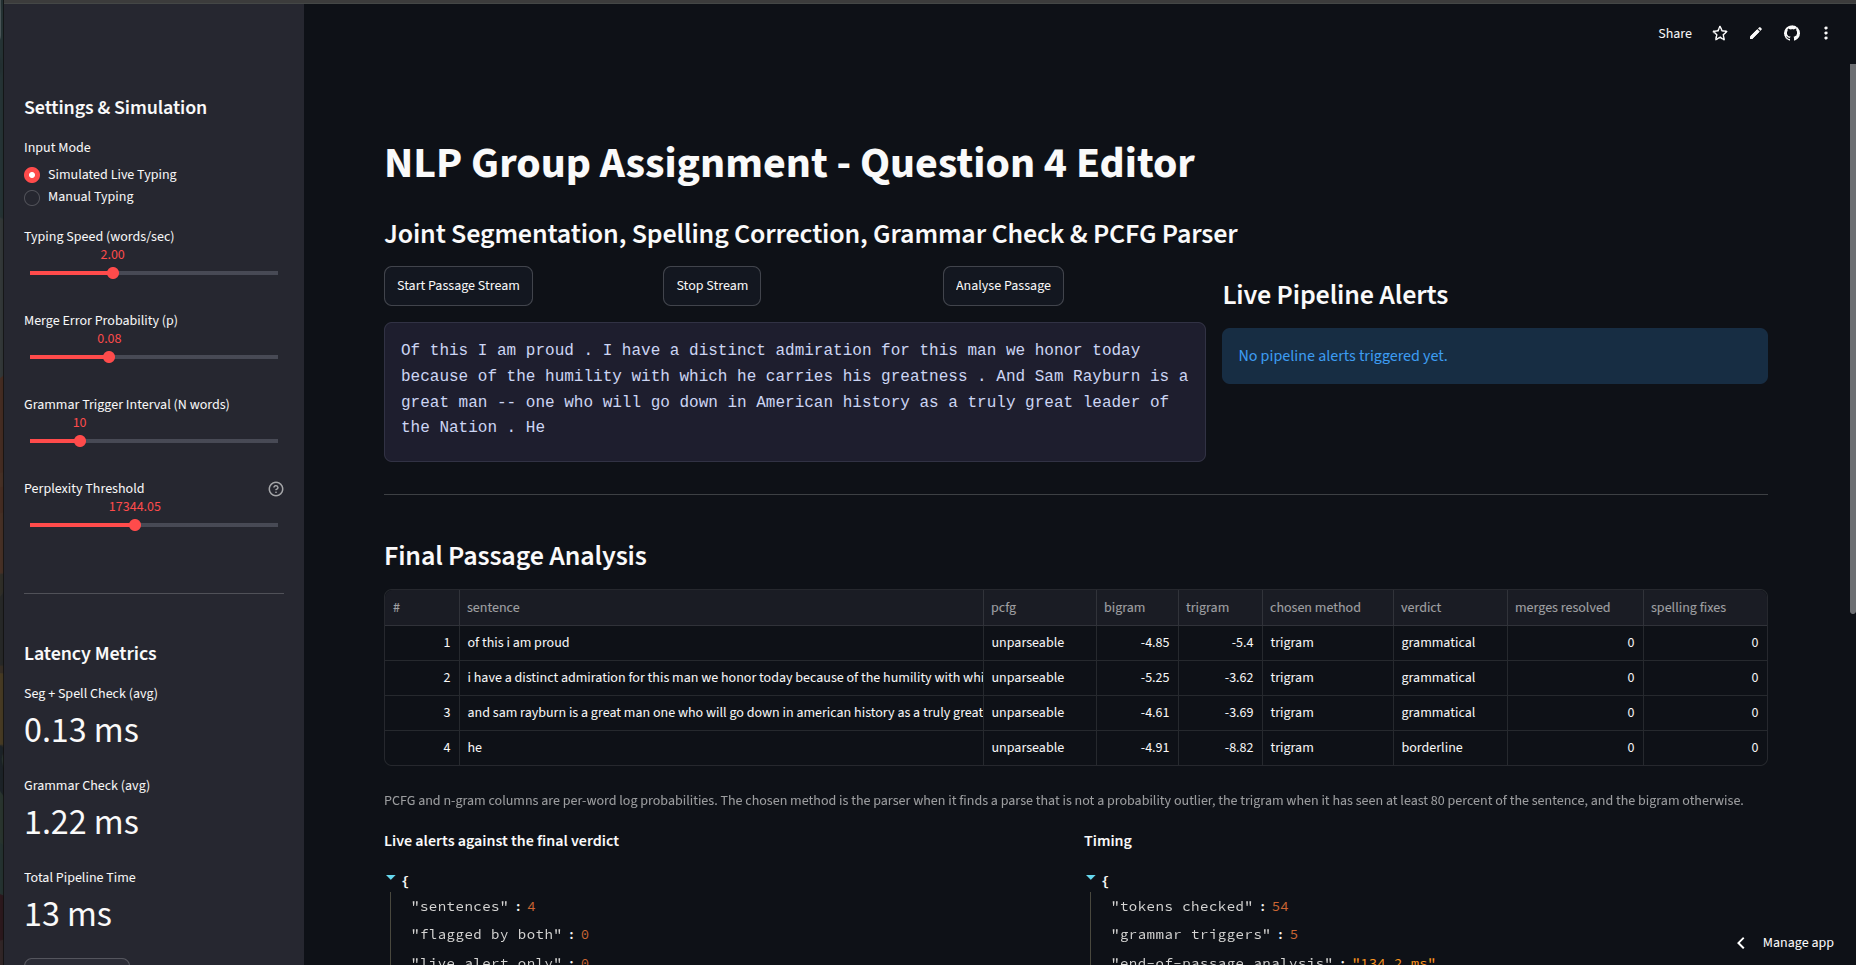
\includegraphics[width=\linewidth]{Question-4/reports/live_app.png}
\caption*{Live alerts in the editor}
\end{figure}

The first screenshot is Simulated Live Typing mode on a Brown passage about Sam Rayburn, after the stream finished and Analyse Passage ran. The Final Passage Analysis table shows all four sentences: the PCFG fails to parse any of them under the pruned grammar, so the method-selection rule (\S{}3) falls back to the trigram for every row, which has full vocabulary coverage on this passage. Three sentences come back grammatical and the one-word sentence 4 (``he'') is borderline. No merges or spelling fixes landed in this run.

\begin{figure}[H]
\centering
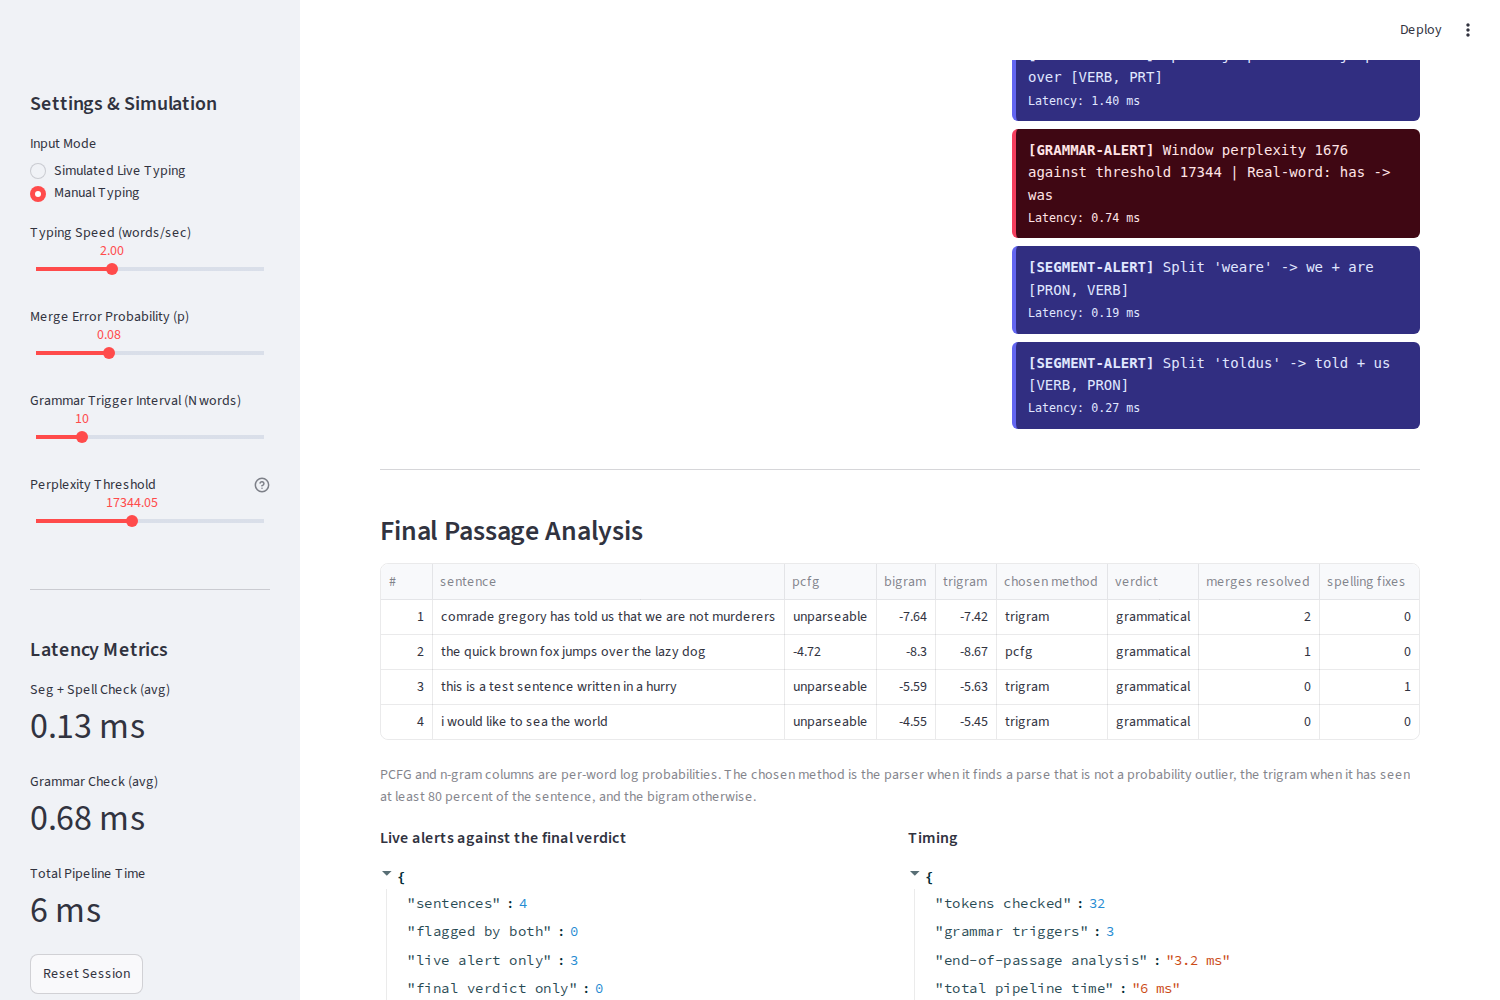
\includegraphics[width=\linewidth]{Question-4/reports/live_app_analysis.png}
\caption*{End of passage analysis}
\end{figure}

The second screenshot is the same session scrolled further down. ``Live alerts against the final verdict'' (\S{}5.1's live metric) shows 3 of the 4 sentences clean under both the live per-token checks and the final verdict, with 1 sentence flagged by the final verdict only --- a 75\% agreement rate. Timing shows 54 tokens streamed, 5 grammar triggers fired, a 134.2 ms end-of-passage analysis, and 13 ms of total live pipeline time. The sidebar's latency metrics (0.13 ms average segmentation+spelling check, 1.22 ms average grammar check) match the numbers in \S{}4. Below that, the PCFG Constituency Parse Trees panel shows why the parser lost every sentence in this run: sentence 1 (``of this i am proud'') is tagged IN DT PRP VBD JJ . and comes back unparseable under the pruned grammar, and sentence 2 is unparseable for the same reason.

\subsection*{8. Limitations}
\addcontentsline{toc}{subsection}{8. Limitations}

\begin{itemize}
\item The pruned grammar is the main limit on the parser. Keeping every production instead of only those seen twice raises the parse rate from 41 percent to 65 percent on a sample of 150 treebank sentences, but the grammar pickle grows to 116 MB, which is over GitHub's file limit, and parsing slows from 34 ms to 1,048 ms per sentence. At a second per sentence the end-of-passage analysis would stop being interactive, so the pruned grammar stays and the decision rule is built to cope with unparseable sentences instead.
\item Very short fragments score well and are called grammatical. A one word sentence such as \texttt{mccormack} has almost nothing to average over, so its per-word score is dominated by the sentence-end probability and lands above the floor.
\item The first parse in a process pays about 200 ms to build the grammar's rule index, and a cold end-of-passage analysis comes in around 700 ms as a result. Every analysis after that in the same session runs in 15 to 50 ms.
\item Add-k is a weak smoother. It is what the brief asks for, and the perplexities in section 1.3 show what it costs compared to the Witten-Bell model Q1 uses for the same corpus.
\item The real-word check produces most of the grammar alerts and most of them are wrong. The 2.0 nat margin comes from Q3 and was tuned for sentence-level correction, not for ten-word windows that can cut across a sentence boundary.
\item Sentences are cut on final punctuation, with a guard for single letter initials. An abbreviation such as \texttt{U.\allowbreak{}S.\allowbreak{}} still splits a sentence in two.
\end{itemize}

\end{document}
